\chapter{Transitional Rayleigh-B\'{e}nard Poiseuille flows}\label{chap:3}

In this chapter, we investigate the transitional flow regimes arising from the interaction between buoyancy and shear in Rayleigh-B\'{e}nard Poiseuille (RBP) flows within large domains.
The transition boundaries between the bistable system consisting of spiral defect chaos (SDC) and ideal straight rolls (ISRs) in Rayleigh-B\'{e}nard convection (see \S \ref{sec:bkgrd_RBC}), and subcritical turbulence in plane Poiseuille flows (see \S \ref{sec:bkgrd_transitional}) are not known.

Using Nektar++, a spectral/\textit{hp} element package, we conduct direct numerical simulations over a range of Rayleigh numbers, $Ra \in [0, 10000]$, Reynolds numbers, $Re \in [0, 2000]$ and unit Prandtl number, we identify five distinct regimes: (1) bistable SDC \& ISRs, (2) ISRs, (3) wavy rolls, (4) intermittent rolls, and (5) shear-driven turbulence.
The newly identified intermittent rolls state, features longitudinal rolls that spontaneously decay towards the laminar state.
In the transitional shear-driven turbulent regime, longitudinal rolls may coexist with turbulent-laminar bands.
The role of longitudinal rolls in transitional RBP flows is apparent, and we examine the unstable manifold of longitudinal rolls in a confined domain, integrating along which led to transient turbulence, decaying towards the laminar state before regenerating into longitudinal rolls again, sustaining transient turbulence.
Near the intermittent roll regime, a periodic orbit emerges between the longitudinal rolls and the laminar state within a confined domain.
Above a certain $Re$ threshold, the unstable longitudinal rolls provide an intermediate pathway for the transition from the laminar state to turbulence.
Finally, we provide a state space sketch of the dynamical processes, emphasising the role of longitudinal rolls in transitional RBP in confined domains, and discuss connections to the large domains.
% 
\section{Objectives}
While the linear stability characteristics of laminar RBP flows have been well studied (see \S \ref{sec:bkgrd_RBP}), the transition to shear-driven turbulence remains and the related nonlinear dynamics remain largely unexplored.
% For instance, how do wavy rolls evolve as $Re$ increases?

% Additionally, we also aim to bridge the gap between RBC (see \S \ref{sec:bkgrd_RBC}), and PPF (see \S \ref{sec:bkgrd_PPF}) by investigating the impact of $Re$ on the bistability between SDC and ISRs in RBC, as well as the influence of $Ra$ on turbulent-laminar bands in PPF.
As the first step towards understanding the transition in RBP flows, the main objective of this chapter is to perform exploratory direct numerical simulations (DNS) of transitional RBP flows while investigating the impact of $Re$ on the bistability between SDC and ISRs in RBC as well as the influence of $Ra$ on turbulent-laminar bands in PPF.
For this purpose, we consider a relatively wide range of parameter space given by $Ra \in [0, 10000]$ and $Re \in [0, 2000]$ at $Pr = 1$ in both large and confined domains ($\Gamma = 4\pi$, $\pi/2$, in particular).
Given that this study is largely exploratory, we will focus on identifying different flow regimes and providing key insights into their dynamical processes.
Due to the large parameter space, we do not intend to perform an extensive bifurcation analysis that involves the computation and analysis of the invariant solutions, which could be computationally very costly, especially in a large domains.

% The main objective of this chapter is to perform direct numerical simulations (DNS) of transitional RBP flows within $Ra \in [0, 10000]$ and $Re \in [0, 2000]$ at $Pr = 1$ in both large and confined domains, $\Gamma = 4\pi$, $\Gamma = \pi/2$.
% This study is largely exploratory, focusing on identifying different flow regimes and providing key insights into their dynamical processes.
% Hence, we do not intend to perform bifurcation analysis due to the lack of prior knowledge of the phase space, which could lead to large computational costs.

The chapter is organised as follows: in \S \ref{sec:rbp_2}, we describe the problem formulation, governing equations, the numerical methods and setup.
In \S \ref{sec:rbp_3}, we present the $Ra$-$Re$ phase space, identifying five distinct regimes and their coarse-grained transition boundaries.
We also show a new `intermittent roll' regime and discuss the coexistence of longitudinal rolls with turbulent-laminar bands, highlighting the role of longitudinal rolls in transitional RBP flows.
In \S \ref{sec:rbp_4}, we perform a numerical experiment, in which simulations are performed along the unstable manifolds of longitudinal rolls in a confined domain, $\Gamma = \pi/2$.
We will see that this reveals some dynamical connections between shear-driven turbulence, longitudinal rolls, and the laminar state and subsequently discuss their relevance to the larger domain.
Finally, we conclude in \S \ref{sec:rbp_5}, and provide some perspectives for future work.

% The paper is organised as follows: in \S \ref{sec:rbp_2}, we describe the problem formulation, governing equations, numerical methods and setup. In \S \ref{sec:rbp_3}, we present the $Ra$-$Re$ phase space, identifying five distinct regimes and their transition boundaries. We also introduce a new `intermittent roll' regime and discuss the coexistence of longitudinal rolls with turbulent-laminar bands, highlighting the role of longitudinal rolls in transitional RBP flows. In \S \ref{sec:4}, we investigate the unstable manifolds of longitudinal rolls in a confined domain, $\Gamma = \pi/2$, revealing dynamical connections between shear-driven turbulence, longitudinal rolls and the laminar state, and discuss its relevance to the larger domain. Finally, we conclude in \S \ref{sec:5}, and propose directions for future work.

% In this $Ra-Re$ phase space, we identify five distinct regimes: (1) bistable SDC \& ISRs, (2) ISRs, (3) wavy rolls, (4) intermittent rolls, and (5) shear-driven turbulence, and describe their transition boundaries.
% We characterise the impact of $Re$ on the bistable system between SDC and ISRs, and discuss the $Re$-threshold where SDC ceases to exist.
% The intermittent rolls represent a new regime, characterised by spatiotemporal intermittent longitudinal rolls.
% As $Re$ approaches the onset of turbulence $Re \sim 1000$, we discuss the coexistence of longitudinal rolls with the spatiotemporal turbulent-laminar bands.
% The spatiotemporal nature of the longitudinal rolls is evident, and we seek to understand its temporal dynamics by restricting the domain size to a confined domain, $\Gamma = \pi/2$ where we discover new dynamical processes which describes the temporal evolution of longituidnal rolls.
% 

% We discussed a new regime, known as intermittent rolls emerging near $Re\sim 500$, characterised by longitudinal rolls with spatiotemporal intermittent behaviour and also the coexistence of longitudinal rolls with turbulent bands near the onset of turbulence $Re \sim 10000$.
% where we identify a new regime known as intermittent rolls described by spatiotemporal intermittent 
% and small domains, $\Gamma = \pi/2$.
% We do not intend to perform a full bifurcation study within this $Ra$-$Re$ parameter space due to the potentially large computational cost associated with this exploration.
% due to not knowing which set of $Ra$-$Re$ parameters to begin with, leading to large computational costs. 
% At $Re = 0$, bistability between SDC and ISRs is expected within this $Ra$ range.
% Starting from small values of $Re$, we explore the impact of shear on the bistable nature of SDC and ISRs.
% As wavy rolls are expected near $Re \sim 100$, 
% 
% 
% 
% We explore the bistable nature of his bistability persists under the influence of a Poiseuille flow as $Re$ is increased.
% We also examine the impact of $Re$ on the stability boundaries of the Busse balloon, and whether its associated secondary instabilities (e.g., oscillatory, skewed-varicose) arise between $0 < Re \leq 10$.
% Subsequently, we investigate the behaviour of wavy rolls at $Re = 100$ as $Re$ increases towards $Re = 1000$, where subcritical shear-driven turbulence is expected.
% Do wavy rolls, reminiscent of optimal streamwise rollers in shear flow \citep{reddy1993energy}, assist the transition towards subcritical turbulence?
% For $Re > 100$, our findings indicate that the wavy rolls break down into a new state known as `intermittent rolls'.
% The intermittent rolls are described by intermittent oscillations between the laminar and longitudinal roll states discussed later.
% As the flow transitions to shear-driven turbulence near $Re \sim 1000$, spatially intermittent turbulent bands are expected.
% In this regime, laminar bands become linearly unstable at $Ra > Ra_{\parallel}$, potentially leading to longitudinal rolls.
% This suggests that the turbulent bands could coexist and interact with neighbouring longitudinal rolls, which are visually present.
% The dynamics of intermittent rolls and the possible interaction of longitudinal rolls and turbulence are complicated, and we focus on the MFU in an attempt to elucidate a simpler description of the dynamics (if possible).
% In the intermittent roll regime, the solution trajectory forms a periodic orbit between the unstable longitudinal roll and the unstable laminar state within an MFU.
% At $Re \sim 1000$, transient turbulence emerges as a chaotic saddle, where the solution trajectory visits the chaotic saddle, unstable longitudinal rolls and laminar state, forming a basin of attraction.
% Finally, as $Re$ approaches $Re = 1600$, turbulence is sustained, and the unstable longitudinal rolls provide a pathway towards turbulence from the unstable laminar state.


% Extended organisation, could be use for conclusions...
% \begin{itemize}
%     \item Section \ref{sec:rbp_2}: Describes the problem formulation, governing equations and numerical methods and setup.
%     \item Section \ref{sec:rbp_3}: Maps the full $Ra$-$Re$ phase space, identifying five distinct states and its boundaries within $Ra \in [0, 10000]$, $Re \in [0, 2000]$ at $Pr = 1$ for $\Gamma = 4\pi$, consisting of (1) SDC \& ISRs, (2) ISRs, (3) wavy rolls, (4) intermittent rolls and (5) shear-driven turbulence. We discuss their common characteristics and whether they are dominated by buoyancy or shear forces (or both), and introduce the new intermittent rolls regime.
%     \item Section \ref{sec:4}: Explores the coexistence of longitudinal rolls and turbulent bands, a challenge addressed through numerical simulations in a minimal flow unit (MFU) and analysis of its state space trajectories. Our findings reveal that the unstable longitudinal rolls lead to transient turbulence, which decays towards the laminar state before re-energising into longitudinal rolls where a basin of attraction is formed - referred to as the `thermally sustained turbulent process'. We then examine the MFU's state space trajectories intermittent regime, where the turbulence ceases to exist, where we observe a periodic orbit emerge between the longitudinal and laminar state. Finally, we extend these dynamics to the large domain.
%     \item Section \ref{sec:5}: Summarises the key findings, and proposed future work.
% \end{itemize}
% The main contributions of this study are summarised as follows,
% \begin{enumerate}
%     \item The documentation of the $Ra$-$Re$ phase space for $Ra \in [0, 10000$, $Re \in [0, 2000]$, where a new intermittent state is discovered.
%     \item A study of the intermittent dynamics between longitudinal rolls, shear-driven turbulence and the laminar state within a small domain $\Gamma = \pi/2$ and its relevance to $\Gamma = 4\pi$.
% \end{enumerate}

\section{Problem formulation}\label{sec:rbp_2}
\subsection{Governing equations}
The motion of fluid flow in an RBP system (see \S \ref{sec:bkgrd_overview}), is govern by the non-dimensionalised Navier-Stokes equations with Boussinesq approximation,
% which describes a layer of fluid sandwiched between two extended parallel plates of equal length and span, $L = L_x =  L_z$, separated by depth, $d$ (or two half heights, $h = d/2$), with a uniform upper and lower plate temperature $T_U$ and $T_L$.
% The fluid is unstably stratified such that $\Delta T = T_L - T_U > 0$. 
% The fluid has a density of $\rho$, kinetic viscosity, $\nu$, thermal diffusivity $\kappa$. The governing equations are the non-dimensionalised Navier-Stokes equations with Boussinesq approximation given by,
\begin{subequations}\label{eq:rbp_RBP}
\begin{equation}
    \frac{\partial \mathbf{u}}{\partial t}  + (\mathbf{u}\cdot \nabla)\mathbf{u} = -\nabla p + \frac{1}{Re}\nabla^2 \mathbf{u} + \frac{Ra}{8PrRe^2}\theta \mathbf{{j}},
\end{equation}
\begin{equation}
    \frac{\partial \theta}{\partial t} + (\mathbf{u} \cdot \nabla)\theta = \frac{1}{RePr} \nabla^2 \theta,
\end{equation}
\begin{equation}
    \nabla \cdot \mathbf{u} = 0,
\end{equation}
\end{subequations}
with the following boundary conditions at the wall,
\begin{equation}
    \mathbf{u}|_{y=\pm h} = 0, \quad \theta|_{y = -h} = 1, \quad \theta|_{y=h} = 0,
\end{equation}
and periodic boundary conditions in the planar $x$ and $z$ directions.
$\mathbf{u}(\mathbf{x},t)$ denotes the non-dimensionalised velocity scaled by the laminar centreline velocity, $W_c$, i.e. $W_{lam}(y)= W_c(1-y^2)$.
$\mathbf{x} = (x,y,z)$ and $t$ denote the non-dimensionalised spatial and temporal coordinates scaled by the half-height, $h$ and the advective time scale, $W_c/h$, where $x, y, z$ refers to the spanwise, wall-normal and streamwise directions, respectively.
$p$ refers to the non-dimensionalised pressure scaled by $\rho W_c^2$, and $\theta(\equiv(T-T_U)/\Delta T)$ refers to the non-dimensionalised temperature with $T$ being the absolute temperature.
$\mathbf{j}$ denotes the unit vector in the $y$-direction. 

We note that the rescaled $Ra/8$ term in the momentum forcing terms is equivalent to the Rayleigh number scaled based on the half-depth, $h$, whereas $Ra$ is scaled based on depth, $d$, as in classical RBC.
The Rayleigh number, $Ra$, Reynolds number $Re$ and Prandtl number, $Pr$ are defined in \S \ref{sec:bkgrd_overview}. 
We set $Pr = 1$ in this study.
For $Re=0$, the Rayleigh-B\'{e}nard convection problem, we note that the equation \eqref{eq:rbp_RBP} becomes singular.
In such cases, we solve the non-dimensionalised incompressible Navier-Stokes equations based on thermal length, velocity and temporal scales given in \S \ref{sec:chap4}.

\subsection{Numerical Methods}
The governing equations are solved numerically using Nektar++, an open-source spectral/\emph{hp}-element package \citep{cantwell_nektar_2015,moxey_nektar_2020}. 
The computational mesh consists of 2D quadrilateral elements in the $x-y$ plane generated using Gmsh \citep{geuzaine_gmsh_2009} and then imported into Nektar++ using Nekmesh \citep{green_nekmesh_2024}.
The spatial domain is discretised based on the quasi-3D approach, employing spectral/\emph{hp} elements in the $x-y$ plane and Fourier expansions in the $z$ (see \S \ref{sec:nm_quasi3d}).
We emphasise that the streamwise direction is in $z$.
The discretised equations are solved using a velocity correction scheme, based on a second-order stiffly splitting scheme, where the nonlinear advection and forcing terms are treated explicitly, while the pressure and diffusion terms are treated implicitly (see \S \ref{sec:nm_vcs}).
The $3/2$ and polynomial de-aliasing rule for the Fourier expansions and spectral/\emph{hp} elements are applied during the evaluation of the nonlinear advection terms.
To drive the flow, we also enforce a constant volumetric flux (see \S \ref{sec:nm_constantflux}).

\subsection{Parametric sweep of $Ra$-$Re$ space}\label{sec:Raresweep}
We consider fifty-two numerical simulations at $Re = 0, 0.1, 1, 10, 100, 500, 750, 1000, 1050$, $2000$, and $Ra = 0, 2000, 3000, 5000, 8000, 10000$ at $Pr = 1$ with a large aspect ratio of $\Gamma = 4\pi$.
Their spatial and temporal numerical resolutions and time-integration horizon, $T$, are described in the Appendix \ref{app:params}.
The initial conditions of all cases are sampled from a statistically stationary solution.
Laminar solutions are obtained for $Ra = 0$, $Re \leq 1000$, with the given set of parameters and are omitted from the analysis.
For all the cases considered here, we maintain the same spatial resolution except $Re = 2000$, where the number of Fourier expansions was doubled.
The temporal resolution between the numerical simulations differs due to time scales arising from the different flow physics, as we shall see later.
We have also considered a mesh independence study for the end case of $Ra = 10000$, $Re = 2000$, where doubling the number of Fourier modes or increasing the polynomial order by 1 led to a $<1\%$ change in near-wall transport properties defined by the Nusselt number, $Nu = -\langle \mathrm{d}\theta/\mathrm{d}y_{y=-1}\rangle_{x,z} d/\Delta T$, and shear, $\langle \mathrm{d}w/\mathrm{d}y|_{y=-1} \rangle_{x,z} $, on the lower wall, where $\langle \cdot \rangle_{x,z} = 1 / (L_xL_z) \int_{z,x} \; \cdot \; \mathrm{d}x\mathrm{d}z$ refer to the plane-averaged operator.
\subsection{Linear Stability Analysis}\label{sec:linearstab}
In \S \ref{sec:rbp_4}, we will perform numerical experiments where small disturbances are added along the unstable manifolds of longitudinal rolls.
This is rooted in linear stability methods discussed earlier in \S \ref{sec:bkgrd_transitional}, and its numerical technique is presented in \S \ref{sec:nm_arnoldi}.
To determine the unstable manifolds, we consider a small disturbance about the longitudinal roll state,
\begin{subequations}\label{eq:rbp_basepert}
\begin{equation}
    \mathbf{u}(\mathbf{x}, t) = \mathbf{u}_{LR}(\mathbf{x}) + \mathbf{\hat{u}}(\mathbf{x}, t),
\end{equation}
\begin{equation}
    \theta(\mathbf{x}, t) =\theta_{LR}(\mathbf{x})  + \hat{\theta}(\mathbf{x}, t), 
\end{equation}
\begin{equation}
    p(\mathbf{x}, t)  = p_{LR}(\mathbf{x})  + \hat{p}(\mathbf{x}, t),
\end{equation}
\end{subequations}
where $\mathbf{q}  = [\mathbf{u}, \theta, p]^T$, $\mathbf{q}_{LR}=[\mathbf{u}_{LR}, \theta_{LR}, p_{LR}]^T$ and $\mathbf{\hat{q}}=[\mathbf{\hat{u}}, \hat{\theta}, \hat{p}]^T$ refers to the solution vector, the longitudinal state and the disturbances respectively.
We substitute equation \eqref{eq:rbp_basepert} into \eqref{eq:rbp_RBP} and neglect the nonlinear terms, leading to the linearised equations,
\begin{subequations}\label{eq:rbp_linearised}
\begin{equation}
    \frac{\partial \mathbf{\hat{q}}}{\partial t} = \mathcal{A}(\mathbf{q}_{LR}; Re, Ra, Pr) \mathbf{\hat{q}}, 
\end{equation}
where
\begin{equation}
\mathcal{A}(\mathbf{q}_{LR}; Re, Ra, Pr) =
    \left(
    \begin{array}{c c c}
      - (\mathbf{u}_{LR} \cdot\nabla) - (\nabla \mathbf{u}_{LR} \; \cdot) + 1/Re \nabla^2 & \frac{Ra}{8Re^2 Pr}\mathbf{\hat{j}} & -\nabla \\
      -(\nabla \theta_{LR} \; \cdot)  &  - (\mathbf{u}_{LR} \cdot \nabla) + \nabla^2 & 0 \\
      \nabla \cdot  & 0  & 0
    \end{array}
    \right).
\end{equation}
\end{subequations}
Consider that the longitudinal rolls are invariant along the $z$-direction, which are also assumed to be periodic in $x$-direction, and the following form of normal-mode solution can be considered,
\begin{equation}\label{eq:rbp_ansatz}
    \mathbf{\hat{q}} (\mathbf{x},t) = \mathbf{\breve{q}}(x,y)e^{i(\alpha x+\beta z)+\lambda t} + \text{c.c},
\end{equation}
where $\lambda, \alpha$ and $\beta$ are the complex frequency, the spanwise wavenumber (or the Floquet exponent), and the stream wavenumber, respectively. Using the periodic nature of $\mathbf{\breve{q}}(x,y)$ in the $x$-direction, (\ref{eq:rbp_ansatz}) can also be written as 
\begin{equation}\label{eq:rbp_simAnsatz}
    \mathbf{\hat{q}} (\mathbf{x},t) = \left[\sum_{n=-\infty}^{\infty}\mathbf{\breve{\breve{q}}}_n(y)e^{i \frac{2\pi}{L_x}(n+\epsilon) x} \right] e^{i\beta z+\lambda t} + \text{c.c},
\end{equation}
where $\epsilon(=\alpha L_x/(2\pi))$ is the Floquet detuning parameter with $0 \leq \epsilon \leq 1/2$.
In this study, we will only consider the identification of the unstable manifolds of longitudinal rolls in a fixed computational domain; therefore, the fundamental mode, $\epsilon = 0$, is of sole interest.
Substituting equation \eqref{eq:rbp_simAnsatz} into (\ref{eq:rbp_linearised}) result to a discretised eigenvalue problem with the eigenvalue $\lambda$. The wavenumber $\beta$, is restricted to discrete values of $\beta=2 \pi m/L_z$, and $m$ is a positive integer for the given computational domain. The resulting eigenvalue problems are solved using an iterative Arnoldi algorithm based on time-stepping schemes implemented in Nektar++ (see \S \ref{sec:nm_arnoldi}).


%%%%%%%%%%%%%%%%%%%%%%%%%
% Ra-Re Phase Space Summary
%%%%%%%%%%%%%%%%%%%%%%%%%
\section{$Ra$-$Re$ phase space}\label{sec:rbp_3}
\subsection{Classification}
\begin{figure}
    \centering
    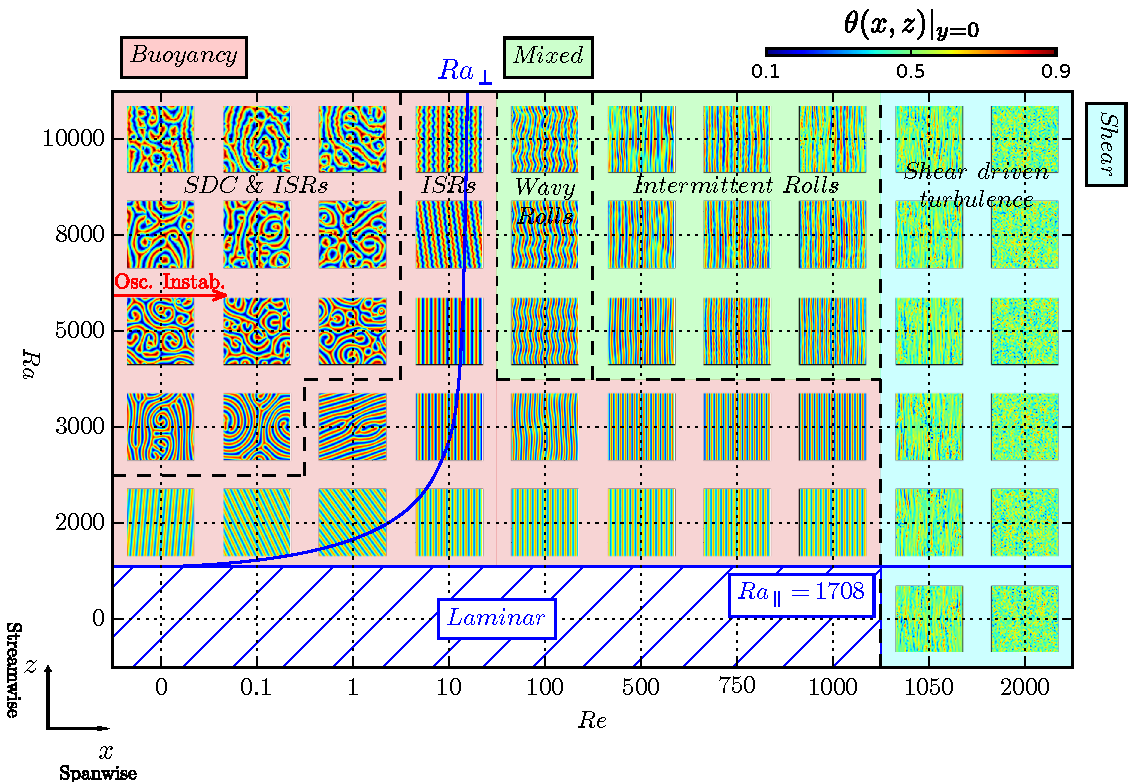
\includegraphics[width=0.9\textwidth]{TransitionalRBP/Figures/PhaseSpace/RaRePhaseSpace.pdf}
    \caption{The $Ra-Re$ phase space illustrates the terminal midplane temperature snapshots, $\theta(x,z)|_{y=0}$ for $Re \in [0,2000]$ and $Ra \in [0, 10000]$, classified into five distinct regimes: (1) SDC \& ISRs, (2) ISRs, (3) wavy rolls, (4) intermittent rolls and (5) shear-driven turbulence. The blue solid curves refer to primary neutral curves of the longitudinal and transverse rolls $Ra_\parallel, Ra_\perp$. The red curve refers to secondary oscillatory instability of ISRs at $Re = 0$ \citep{bodenschatz_recent_2000}. Shades of red, green and blue indicate their dominant mechanism, whether driven by buoyancy or shear (or mixed). The plot is not to scale.}
    \label{fig:rarephase}
\end{figure}

We present the results obtained from the DNS of transitional RBP flows, focusing on the parameter space defined by Rayleigh numbers in the range $Ra \in [0, 10000]$, and Reynolds numbers in the range of $Re \in [0, 2000]$ (see Appendix \ref{app:params} for the full details).
At the two end points of the $Re$-spectrum considered (i.e. $Re = 0, 2000$), SDC and subcritical shear-driven turbulence appear.
Figure \ref{fig:rarephase} shows the snapshots of the midplane temperature, $\theta(x,z)|_{y=0}$, of different flow regimes on the $Ra$-$Re$ phase space.
The solid blue curves represents to the neutral stability boundaries for the longitudinal and transverse rolls as $Ra_\parallel = 1708$ and $Ra_\perp = f(Re)$, respectively \citep{gage_stability_1968}.
In the absence of shear at $Re=0$, these curves merge into the classical critical RBC instability at $Ra_{c} = 1708$, as ISRs become rotationally invariant about the wall-normal axis.
Furthermore, a red arrow roughly indicates the secondary neutral stability boundary, marking the onset of oscillatory instabilities of ISRs within $5000 < Ra < 8000$ at $Re = 0$ \citep{clever_transition_1974}.
We note that the phase diagram in figure \ref{fig:rarephase} is not plotted to scale precisely but serves as a conceptual reference to distinugish between different flow states.

In this $Ra$-$Re$ phase space, we categorise the flow behaviour into five distinct regimes: (1) bistability between SDC and ISRs (SDC \& ISRs), (2) ideal straight rolls (ISRs), (3) wavy rolls, (4) intermittent rolls, and (5) shear-driven turbulence.
The categories are defined based on common flow structures (patterns), and/or dynamical characteristics, ranging from equilibrium solutions to intermittent and chaotic dynamics.
Furthermore, we classify these states based on their first and second-order statistical properties, where they appear independent of $Re$ in the buoyancy-dominated regime (shaded in red), and $Ra$ in the shear-dominated regime (shaded in blue), discussed in Appendix \ref{app:statistics}.
In the mixed regime shaded in green, both $Ra$ and $Re$ are important.
% The mixed regime flows (green shading), where both $Ra$ and $Re$ influence the statistics significantly (see Appendix \ref{app:statistics}).

In the buoyancy-dominated regime, the flow structures are predominantly organised by convection rolls, such as SDC, transverse, oblique, longitudinal rolls (and ISRs with no mean flow), or oscillatory rolls.
The bistability between SDC and ISRs is preserved for $Ra \geq 3000$ at $Re = 0.1$, and $Re = 1$ for $Ra \geq 5000$.
This points towards the existence of $Re$, at which SDC disappears, say $Re_s$, 
$Re_s$ appears to depend on $Ra$, as demarcated by the black dashed lines on the left side of figure \ref{fig:rarephase}.
However, computing this $Re_s$-threshold is beyond the scope of this thesis.

Notably, a transverse roll with a `hooked-like' defect is observed at $Re = 1$, $Ra = 3000$, reminiscent of the multiple `non-ISR' states in RBC (see references in \S \ref{sec:bkgrd_RBC}).
At $Re = 10$, SDC disappears and longitudinal rolls appear.
As $Re$ is increased further to $1000$, the longitudinal rolls emerge as the preferred solution at $Ra = 2000, 3000$.
% Indeed, the growth rates for the onset of longitudinal rolls become dominant compared to those of oblique/transverse rolls as $Re$ is increased \citep{gage_Reid_1968}.
Notably, the non-dimensionalised spanwise wavenumber of these longitudinal rolls is approximately $\alpha d \approx 1.65$, which happens to lie outside of the stability boundaries of the Busse balloon in RBC \citep{busse_non-linear_1978}.
This suggests that the stability boundaries of the longitudinal rolls may expand as $Re$ increases.
% Further evidence comes from the skewed-varicose longitudinal roll structure at $Re = 100$, $Ra = 3000$, which resembles a skewed-varicose instability, a secondary instability related to the Busse balloon boundaries \citep{Busse_Clever_1979}.

As $Re$ approaches $100$, the longitudinal rolls undergo a secondary wavy instability \citep{clever_instabilities_1991, pabiou_wavy_2005, nicolas_characterisation_2010}, leading to the emergence of wavy longitudinal rolls depicted in figure \ref{fig:rarephase}.
The wavelength of the streamwise waviness and the spanwise periodic longitudinal roll appear to be approximately three intervals of streamwise length, $\Lambda_z \sim L_z / 3$, and twelve intervals of spanwise length, $\Lambda_x \sim L_x/12$, respectively.
The ratio between the wavelength of streamwise waviness and spanwise roll is about $\sim 4$, around the ballpark reported by \cite{clever_instabilities_1991}.

% \begin{figure}
%     \centering
%     \includegraphics[width=\linewidth]{TransitionalRBP/Figures/PhaseSpace/theta_hat-compiled.pdf}
%     \caption{The time-averaged spatial planar $x$-$z$ wavenumber spectra of midplane perturbation temperature, $\frac{1}{T} \sum_T |\widehat{\theta'|_{y=0}}(n_x,n_z,t)|$ at $Re = 100,10$, (a,e) $Ra = 3000$, (b,f) $Ra = 5000$, (c,g) $Ra = 8000$, (d,h) $Ra = 10000$. The coefficient is defined by taking the Fourier transform of the instanteneous midplane perturbation temperature $\widehat{\theta'|_{y=0}}(n_x,n_z,t) = \int_{x,z} \theta'|_{y=0}(x,z,t) e^{-i(\alpha n_x x + \beta n_z z)} \; \mathrm{d}x \mathrm{d}z$ where $\alpha = 2\pi/L_x$ and $\beta = 2\pi/L_z$. The coefficients obey the conjugate symmetry, i.e $\widehat{\theta'|_{y=0}}(n_x,n_z,t)=\widehat{\theta'|_{y=0}}^*(-n_x,-n_z,t)$}
%     \label{fig:rollspectra}
% \end{figure}

\subsection{Spatiotemporal intermittent rolls}\label{sec:intermittentrolls}
\begin{figure}
    \centering
    \includegraphics[width=\linewidth]{TransitionalRBP/Figures/PhaseSpace/Ra8000-Re500-BotSpaceTime-TimeHist.pdf}
    \caption{The intermittent rolls regime at $Ra = 8000, Re = 500$, $t \in [0, 10000]$. The time history of (a) Nusselt number, and shear, (b) near-wall wall-normal and spanwise perturbation kinetic energy, (c) midplane temperature spacetime plot, and their corresponding near-wall and midplane temporal planar snapshots at (d,e) $t = 3736$, (f,g) $t = 6189$, and (h,i) $t = 8680$.}
    \label{fig:Ra8k-Re500-IntRolls}
\end{figure}

As $Re$ approaches $Re = 500$, the wavy rolls disappear.
Instead, a new regime, referred to as intermittent rolls, is observed.
In this regime, the longitudinal rolls remain as the dominant convection structure, interspersed with a spatio-temporal intermittent breakdown towards the laminar state.
For $Ra = 8000, Re = 500$, this behaviour is illustrated with figure \ref{fig:Ra8k-Re500-IntRolls}(a), where the temporal oscillations of the as the plane-averaged shear rate on the lower wall, $\langle \mathrm{d}w/\mathrm{d}y|_{y=-1} \rangle_{x,z} $, and the Nusselt number, $Nu$.
We note that the plane-averaged shear rate and Nusselt number for the laminar state is at 2 and 1 respectively. 

The spatio-temporal intermittent breakdown of the longitudinal rolls towards the laminar state is observed in figure \ref{fig:Ra8k-Re500-IntRolls}(b), where the bright and dark regions in the space-time plot of near-wall spanwise and wall-normal perturbation kinetic energy, $\mathcal{E}_{u'+v'} = 1/2\left[ u'|_{(y^+,z)=(15,8\pi)}^2 + v'|_{(y^+,z)=(15,8\pi)}^2 \right]$ (where $\mathbf{u}' = \mathbf{u} - W_{lam}(y)$, $y^+ = u_\tau y_0 / \nu$, $u_\tau = \sqrt{\langle \gamma/h \rangle_{t}}$, $y_0 = h - y = 0.44$,  refer to perturbation velocities, dimensionless height, frictional velocity, wall-normal height respectively), highlight the presence of longitudinal rolls and spatially-localised laminar states.
A similar obserbation is made with the space-time plot of midplane temperature, $\theta|_{(y,z)=(0,8\pi)}$, where elongated red/blue lines correspond to regions of longitudinal rolls, while green spots indicate spatially-localised laminar states, highlighting the breakdown process.
The near-wall transport properties, such as the Nusselt number and shear, exhibit strong correlations, peaking at $t = 3736$, corresponding to a spatially coherent longitudinal roll structure in figure \ref{fig:Ra8k-Re500-IntRolls}(d,e).
This is followed by a dip at $t = 6189$ and $t=8680$, indicative of the breakdown towards the laminar state shown in figures \ref{fig:Ra8k-Re500-IntRolls}(f,g) and \ref{fig:Ra8k-Re500-IntRolls}(h,i) respectively.
In other words, the longitudinal rolls enhance heat and momentum transfer across the wall, which is briefly disrupted by its breakdown towards the laminar state.
However, exploring the spatiotemporal intermittency of this regime remains challenging in a large extended domain, 
To overcome this challenge, we consider a confined domain, $\Gamma = \pi / 2$, where spatial intermittency could be artificially suppressed and discuss its temporal intermittent dynamics in \S \ref{sec:IntConfined}.

\subsection{Coexistence with turbulent bands}\label{sec:rbp_3.3}
\begin{figure}
    \centering
    \includegraphics[width=\linewidth]{TransitionalRBP/Figures/RaEffectOnTurbulence/Ra0-Re1050-3-BotSpaceTime-Lows.pdf}
    \caption{Shear-driven turbulence regime at $Ra = 0, Re = 1050$, $t \in [0, 8000]$. Spacetime plots of (a) near-wall wall-normal and spanwise perturbation kinetic energy, (b) midplane temperature spacetime plot, and near-wall and midplane temporal planar snapshots at (c,d) $t = 1100$, (e,f) $t = 4491$, and (g,h) $t = 6171$, highlighting a prolonged laminar patch.}
    \label{fig:spacetime-Ra0k-Re1.05k}
\end{figure}
As $Re$ approaches $Re = 1050$, shear-driven turbulence emerges as spatiotemporal intermittent turbulent-laminar bands, where turbulent and laminar regions can coexist (see references in \S \ref{sec:bkgrd_transitional}).
In the absence of buoyancy ($Ra = 0$), these bands emerge clearly, as shown in figure \ref{fig:spacetime-Ra0k-Re1.05k}.
The spacetime plot of the near-wall wall-normal and spanwise perturbation kinetic energy, $\mathcal{E}_{u'+v'}$, in figure \ref{fig:spacetime-Ra0k-Re1.05k}(a) highlights this coexistence, where the turbulent and laminar regions are indicated by dark and bright areas, respectively.
Notably, a period of prolonged laminar state is observed at $t = 1100, 4491, 6171$, represented by localised green regions in the midplane temperature spacetime plot, $\theta|_{(y,z)=(0,8\pi)}$, in figure \ref{fig:spacetime-Ra0k-Re1.05k}(b).
The prolonged laminar states are also evident in the near-wall and midplane temporal snapshots of figures \ref{fig:spacetime-Ra0k-Re1.05k}(c-h), shown as large pockets of dark and green regions filling approximately half of the spatial domain.
Next, we consider the influence of buoyancy on the turbulent-laminar bands and compare cases at $Ra = 0$ and $Ra = 10000$ at $Re = 1050$.
% The impact of $Ra$ on the nature of turbulent-laminar bands remains unclear.
% For instance, do longitudinal rolls emerge within laminar bands at $Ra > Ra_\parallel$?
% The emergence of longitudinal rolls suggests potential interactions and/or coexistence with neighbouring turbulent bands.
% In this section, we focus on the impact of $Ra$ on turbulent-laminar bands at $Re = 1050$, close to the subcritical shear-driven transition $Re$ for turbulence (see figure \ref{fig:rarephase}).
% We explore the role of longitudinal rolls, and their impact on turbulent-laminar bands, i.e. do longitudinal rolls appear within laminar bands at $Ra > Ra_{\parallel}$ and do they coexist with turbulent bands?
% We compare two numerical experiments, $Ra = 10000, 0$ at $Re = 1050$.
% We present the spacetime graph of the near-wall wall-normal and spanwise perturbation kinetic energy,$\frac{1}{2W_c}|u'+ v'|_{(y^+, z) = (15,8\pi)}$, and midplane temperature plots, $\theta(x,t)|_{y=0}$, and 3 pairs of $x-z$ planar snapshots at different times for $Ra = 10000, 0$, $Ra = 1050$ in figures \ref{fig:spacetime-Ra10k-Re1.05k} and \ref{fig:spacetime-Ra0k-Re1.05k} respectively.
\begin{figure}
    \centering
    \includegraphics[width=\linewidth]{TransitionalRBP/Figures/RaEffectOnTurbulence/Ra10000-Re1050-BotSpaceTime-Highs.pdf}
    \caption{Shear-driven turbulence regime at $Ra = 100000, Re = 1050$, $t \in [0, 8000]$. Spacetime plots of (a) near-wall wall-normal and spanwise perturbation kinetic energy, (b) midplane temperature spacetime plot, and their corresponding near-wall and midplane temporal $x-z$ planar snapshots at (c,d) $t = 1282$, (e,f) $t = 5077$, and (g,h) $t = 6358$, highlighting the coexistence of longitudinal rolls and turbulent bands.}
    \label{fig:spacetime-Ra10k-Re1.05k}
\end{figure}
At $Ra = 10000$, the features of the turbulent-laminar bands appearing as alternate dark and bright bands are visually consistent in the spacetime plot of near-wall wall-normal and spanwise perturbation kinetic energy, $\mathcal{E}_{u'+v'}$, in figure \ref{fig:spacetime-Ra10k-Re1.05k}(a).
% The near-wall wall-normal and spanwise perturbation kinetic energy in the spacetime plot for $Ra = 10000$ in figure \ref{fig:spacetime-Ra10k-Re1.05k}(a) exhibits similar turbulent-laminar band structures
However, key differences between the $Ra = 0$ case emerge.
Notably, the midplane temperature snapshots, $\theta|_{(y,z)=(0,8\pi)}$, at $t = 1282, 5077, 6358$ in figures \ref{fig:spacetime-Ra10k-Re1.05k}(d,f,g) reveal localised regions of streamwise-aligned red and blue stripes, indicating the presence of longitudinal rolls, which are absent in $Ra = 0$.
These longitudinal roll regions are located next to neighbouring turbulent (bright) regions in the near-wall perturbation kinetic energy snapshots in figures \ref{fig:spacetime-Ra10k-Re1.05k}(c,e,g), suggesting that longitudinal rolls coexist with turbulent patches at $Ra = 10000$.
However, we caution that similar red and blue stripes are also observed in $Ra = 0$, where longitudinal rolls are not expected, likely suggesting the presence of quasi-streamwise rollers, shown in figure \ref{fig:spacetime-Ra0k-Re1.05k}(f).
Nonetheless, turbulence occurs more spatially intermittently at $Ra = 0$, containing prolonged pockets of laminar regions, while the turbulent-laminar bands at $Ra = 10000$ appear more visibly consistently (compare figures \ref{fig:spacetime-Ra0k-Re1.05k}(a) and \ref{fig:spacetime-Ra10k-Re1.05k}(a)).
In other words, the presence of longitudinal rolls may promote turbulence locally, where prolonged regions of laminar patches do not appear.
However, investigating this remains challenging due to the spatiotemporal nature of a large extended domain.
To address this, we focus our analysis to a confined domain, $\Gamma = \pi / 2$, where turbulent bands and longitudinal bands cannot coexist, thereby reducing spatial intermittency discussed further in \S \ref{sec:4}.

% This suggests that longitudinal rolls, emerging from the linearly unstable laminar state, might play a role in sustaining turbulence.
% At $Ra = 0$, the turbulent-laminar bands appear more spatially intermittent, where prolonged regions of localised non-turbulent patches emerge near $t = 1100, 6171$, shown as dark and green patches in figures \ref{fig:spacetime-Ra0k-Re1.05k}(a,b).
% Due to the spatial-temporal complexity of the coexistence between longitudinal rolls and turbulence at $Ra = 10000$, it may be challenging to establish connections between them.
% As such, we consider investigate the dynamics within an MFU, where longitudinal rolls and turbulence could be spatially localised.
% For instance, do longitudinal rolls transition to turbulence locally?
% In the  alised regions of alternating elongated hot (red) and cold (blue) stripes within $tU_c/h \in (1400, 1500)$, $x \in (6\pi, 10\pi)$ and $tU_c/h \in (1500, 2000)$, $x \in (0, 4\pi)$ in the midplane temperature spacetime plots of figures \ref{fig:spacetime-Ra10k-Re1.05k}(b) and \ref{fig:spacetime-Ra2k-Re1.05k}(b) respectively, hinting at the presence of longitudinal rolls.
% These elongated hot and cold stripes along the midplane are not to be confused with turbulent streaks which reside near the wall.
% Indeed, we observe patches of longitudinal rolls from the midplane temperature snapshots of figures \ref{fig:spacetime-Ra10k-Re1.05k}(d,f,h) and \ref{fig:spacetime-Ra2k-Re1.05k}(d,f,h), visually differing from the snapshots of $Re = 1800$ (compare with figures \ref{fig:spacetime-Ra10k-Re1.8k}(d,f,h) and \ref{fig:spacetime-Ra2k-Re1.8k}(d,f,h)).
% Interestingly, the longitudinal rolls appear spatially localised, co-existing with neighbouring patches of spatially localised turbulence, consistent in both simulations.
% A subtle difference between the simulations lies in the `uniformity' of the turbulent-laminar bands. 

% For $Ra = 10000$, the turbulent bands appear spatially and temporally uniform, repeating in regular intervals.
% However, at $Ra = 2000$, the turbulent-laminar bands appear to be less uniform, with a prolonged laminar (darkened) patch within $tU_c/h \in (2000, 2500), x \in (6\pi, 8\pi)$ (see figures \ref{fig:spacetime-Ra2k-Re1.05k}(a,b) and the snapshot at $tU_c/h = 2250$ in figures \ref{fig:spacetime-Ra2k-Re1.05k}(g,h)).
% Furthermore, we consider simulations with $Ra = 10000, 0$, where the onset of longitudinal rolls could be precisely controlled.

\section{The role of longitudinal rolls}\label{sec:rbp_4}
\subsection{The thermally-assisted sustaining process (TASP) in a confined domain}\label{sec:TASP}
\begin{figure}
    \centering
    \includegraphics[width=\linewidth]{TransitionalRBP/Figures/RaEffectOnTurbulence/Ra10000-Re1050-MidBotTimeHist.png}
    \caption{Intermittent dynamics in a confined domain at $Ra = 10000$, $Re = 1050$, $t\in[0,3000]$, $\Gamma = \pi/2$. The time history of the (a) Nusselt number and shear. Temporal snapshots of volumetric temperature, planar near-wall streamwise and spanwise perturbations at (b) $t = 1291.5$, (c) $t = 1480.5$, (d) $t = 1564.5$, (e) $t = 1711.5$. Longitudinal rolls and transient turbulence are observed at (b,d) and (c,e), respectively.}
    \label{fig:Ra10k-Re1050-small}
\end{figure}

Motivated by the minimal flow unit (MFU) approach to study turbulence \citep{jimenez_moin_1991}, we consider simulations confined to a confined domain defined by $\Gamma = \pi/2$, where the longitudinal rolls and localised turbulence could be spatially isolated.
We first consider a numerical simulation at $Ra = 10000, Re=1050$, in $\Gamma = \pi/2$, time integrated for $t \in [0, 3000]$.
The initial condition has been sampled from a statistically stationary turbulent field at $Re = 2000$, which is then lowered slowly to $Re = 1050$.
The time history from $t \in [0, 3000]$ of the near-wall transport properties such as the Nusselt number, $Nu$, shear, $\langle \mathrm{d}w/\mathrm{d}y|_{y=-h}\rangle_{x,z}$, volumetric temperature, $\theta(\mathbf{x})$, and near-wall streamwise and spanwise perturbation velocities snapshots, $w'|_{y^+= 15}, v'|_{y^+=15}$, are presented in figure \ref{fig:Ra10k-Re1050-small}.
In this confined domain, the dynamics of the system exhibit temporal intermittency, where the solution trajectory appears to wander between the longitudinal rolls and turbulent dynamics, marked by high and low near-wall transport properties, respectively.
The turbulent dynamics mentioned here refer to chaotic trajectories (see \S \ref{sec:PPF}) marked by a disordered volumetric temperature field and high near-wall transport quantities.

Starting from a longitudinal roll state of spanwise wavenumber of $\alpha d = 4$ at $t = 1291.5$ in figure \ref{fig:Ra10k-Re1050-small}(b), the solution erupts into turbulence at $t = 1480.5$, marked by a disordered temperature field in figure \ref{fig:Ra10k-Re1050-small}(c).
During this breakdown, the near-wall snapshots of streamwise perturbation velocity, $w'|_{y^+ = 15}$, and wall-normal perturbation velocity, $v'|_{y^+ = 15}$, illustrated in the bottom panels of figures \ref{fig:Ra10k-Re1050-small}(c), reveal three pairs of high- and low-speed streaks, each with an average spanwise wavelength of $\Lambda_x^+ \approx 339/3 = 113$ (where $\Lambda_x^+ = u_\tau \Lambda_x / \nu$ refers to non-dimensionalised wavelength), close to the mean streak spacing ($\Lambda^+ \sim 100$) commonly reported in shear flow turbulence \citep{kline_1967,Smith_1983,Kim_Moin_Moser_1987,hkw_1995}.
These streaks appear to be meandering, negatively correlated with wall-normal perturbation velocities, reminiscent of a streak breakdown process \citep{hkw_1995}, or a bursting event \citep{Kim_Kline_Reynolds_1971}, where high- and low-speed streaks are brought close to and away from the wall, respectively, enhancing near-wall transport quantities.
Indeed, this is reflected by large increments of the Nusselt number and shear of roughly $40\%$ at $t = 1480.5$ in figure \ref{fig:Ra10k-Re1050-small}(a).
Subsequently, the solution trajectory returns to a longitudinal roll state at $t=1564.5$, before erupting into turbulence at $t = 1711.5$ (see figures \ref{fig:Ra10k-Re1050-small}(d,e) respectively).
This suggests that the turbulence has a finite lifetime, occurring transiently before decaying towards the laminar state at $Re = 1050$ \citep{hof_2006, schneider_2007}, which is linearly unstable, leading to the onset of longitudinal rolls where transient turbulence could be re-excited again.
% It is likely that this temporal intermittency, described by the oscillation between turbulent dynamics and the longitudinal rolls, occurs as an intrinsic dynamical state in $Ra = 10000, Re = 1050$, when confined to $\Gamma = \pi / 2$.
% Inspired by the lift-up effect as a mechanism to sustain turbulence \citep{brandt2014lift}, we suggest that the longitudinal rolls could redistribute the streamwise mean momentum, providing an alternate mechanism towards turbulence.
% However, turbulence appears to have a finite lifetime, before decaying into longitudinal rolls where a cycle between longitudinal rolls and turbulence could be observed.
% In this case, we hypothesize that the longitudinal rolls at $Ra = 10000$ promote a mechanism for transition to turbulence, in which turbulence may not be sustained at $Re = 1050$ independe , ultimately decaying into the laminar state where the longitudinal rolls are then excited again, forming a thermally-sustaining turbulent mechanism.

\begin{figure}
    \centering
    \includegraphics[width=\linewidth]{TransitionalRBP/Figures/RaEffectOnTurbulence/Ra0-Re1050-MidBotTimeHist.png}
    \caption{Relaminarisation in a confined domain at $Ra = 0$, $Re = 1050$, $t\in[0,3000]$, $\Gamma = \pi/2$. The time history of the (a) Nusselt number and shear. Temporal snapshots of volumetric temperature at (b) $t = 31.5$, (c) $t = 63$, (d) $t = 157.5$, (e) $t = 672$.}
    \label{fig:Ra0k-Re1050-small}
\end{figure}

To test this hypothesis, we consider a numerical simulation at $Ra = 0$, $Re = 1050$, in $\Gamma = \pi / 2$, where longitudinal rolls cannot appear.
The initial condition is taken from a stationary turbulent solution at $Ra = 0$, $Re = 2000$, which is then lowered slowly to $Re = 1050$, and then time integrated for $t \in [0, 700]$.
The time history of Nusselt number, $Nu$, shear, $\langle \mathrm{d}w/\mathrm{d}y|_{y=-h}\rangle_{x,z}$, and the volumetric temperature snapshots, $\theta(\mathbf{x})$, are reported in figure \ref{fig:Ra0k-Re1050-small}.
% Starting from $t = 31.5$, a localised patch of turbulence appears in $x^+,z^+ \in [0, 164]$ in figure \ref{fig:Ra0k-Re1050-small}(c), the turbulent patch subsequently decays, ultimately settling into a laminar state at $t = 630$ in figure \ref{fig:Ra0k-Re1050-small}(e).
Turbulence occurs transiently, which decays towards the laminar solution in $t \in [0, 700]$ within the confined domain.
As we compare the results between $Ra = 0$ and $Ra = 10000$, we propose that the longitudinal rolls at $Ra= 10000$ could provide a transition mechanism towards transient turbulence, which could be sustained indefinitely.

\begin{figure}
    \centering
    \includegraphics[width=\linewidth]{TransitionalRBP/Figures/RaEffectOnTurbulence/T1620-MidBotTimeHist-Quenched-Annotated.pdf}
    \caption{$Ra$-quenching experiments for $Ra = 8000, 5000, 3000, 2000$, $Re = 1050$, $\Gamma = \pi/2$, $t \in [850.5, 5000]$. The time history of (a) shear and (b) volumetric temperature snapshots of the initial condition at $t = 850.5$. Volumetric temperature snapshots for $Ra = 8000$ at (c,d) $t = 1312.5, 1743$, and $Ra = 5000$ at (e,f) $t = 1312.5, 3570$, revealing a longitudinal roll and a turbulent state, respectively. Stable longitudinal rolls emerge for $Ra = 3000$ at (g,h) $t = 1312.5, 4200$, and $Ra = 2000$ at (j,k) $t = 1312.5, 4200$.}
    \label{fig:RaQuench}
\end{figure}
% While, we have only considered the end cases of $Ra = 10000,0$ and the impact of the range of $Ra \in (0, 10000$ on this transition mechanism remains unclear.
% For instance, there could be a critical $Ra > Ra_{c,sec}$ which transition occurs.
% To investigate this further, we performed four numerical experiments in which an initial condition is taken at $Ra = 10000, Re = 1050$, $tU_c/h = 850.5$ (see figure \ref{fig:Ra10k-Re1050-small}, before the onset of longitudinal rolls) whereby $Ra$ is instantly reduced from $Ra = 10000$ to $Ra = 8000, 5000, 3000,2000$.

Next, we investigate the impact of longitudinal rolls on this proposed mechanism at different $Ra$.
We perform four numerical simulations with an initial condition taken from $Ra = 10000, Re = 1050$, at $t = 850.5$ (before the onset of longitudinal rolls, see figure \ref{fig:Ra10k-Re1050-small}), which is lowered instantaneously to $Ra = 8000, 5000, 3000, 2000$ respectively.
The initial conditions are time-integrated further to $t \in [850.5, 5000]$, and the time history of the shear, $\langle \mathrm{d}w/\mathrm{d}y|_{y=-h}\rangle_{x,z}$, and the temperature volumetric temporal snapshots, $\theta(\mathbf{x})$, of these `Ra-quenching' experiment are presented in figure \ref{fig:RaQuench}.
The time history of shear is visibly intermittent for $Ra = 8000, 5000$, depicted as the orange and green trajectories in figure \ref{fig:RaQuench}(a), similar to $Ra = 10000$.
At $Ra= 8000, 5000$, the longitudinal rolls emerge at $t = 1312.5$ (see figures \ref{fig:RaQuench}(d,f)), before erupting into turbulence at $t = 1743$ and $t = 3570$ in figures \ref{fig:RaQuench}(e,g) respectively.
This is then accompanied by a large spike in the near-wall transport properties before dipping briefly in figure \ref{fig:RaQuench}(a).
As $Ra$ is lowered to $Ra = 3000, 2000$, the transients begin to decay into a longitudinal state from $t = 850.5$ to $t = 1312.5$, which remains asymptotically stable until $t = 4200$, represented as the red and purple trajectories of figures \ref{fig:RaQuench}(i,k) respectively. 
This suggests that the longitudinal rolls become linearly unstable for $Ra = 8000, 5000$, leading to turbulence, while remaining stable for $Ra = 3000,2000$.
Notably, the longitudinal rolls state at $Ra = 5000$ remained saturated over a longer period $t \in [1500, 3400]$ (green curve of figure \ref{fig:RaQuench}), suggesting an underlying linear instability with a smaller growth rate compared to $Ra =  8000$.
We note that the longitudinal rolls in figure \ref{fig:RaQuench} have a spanwise wavenumber of $\alpha d=4$, which corresponds to the wavenumber of the dominant primary instability (see Appendix \ref{app:long-pri}), indicating that it is the preferred wavenumber within the confined domain.

% This suggests a critical $Ra$ within $Ra \in (3000,5000)$ where the longitudinal rolls become linear unstable.
% Compared to $Ra = 8000, 10000$, the quiescent region of $Ra =5000$, extends over a visibly longer period $tW_c/h \in (1500, 3400)$ (green curve of figures \ref{fig:RaQuench}), landing support for different perturbation growth rates arising from linear instability.
% The results likely point towards a possible critical $Ra_{c,sec}$, where longitudinal rolls may become linearly unstable, subsequently transitioning into turbulence for $Ra > Ra_{c,sec}$.

\begin{figure}
    \centering
    \includegraphics[width=\linewidth]{TransitionalRBP/Figures/RaEffectOnTurbulence/ev-compiled.pdf}
    \caption{The growth rates of infinitesimal perturbations linearised about longitudinal rolls, $\mathbf{q}_{LR}$, of spanwise wavenumber of $\alpha d = 4$, against (a) streamwise wavenumber $\lambda$, and (b) $Ra$ for $\beta d =1$. The hatches in (a) refer to wavenumbers smaller than those admissible in $\Gamma = \pi/2$. The dash-dotted line in (b) is a standard quadratic regression yielding $Ra_{s}\approx 4720$.}
    \label{fig:SecStabLongRolls}
\end{figure}

To determine the stability characteristics of the longitudinal rolls, we perform linear stability analysis about the longitudinal roll state ($\alpha d= 4$), at $Ra = 10000, 8000, 5000, 3000, 2000$.
The details of linear stability analysis are described in \S\ref{sec:linearstab}, where $\lambda$ and $\mathbf{\hat{s}_\beta}e^{i\beta z}$ refer to the eigenvalue and eigenmode.
The longitudinal roll (base) states, $\mathbf{q}_{LR}$, are obtained by time integrating an initial condition consisting of the laminar (conduction) state, superimposed by the primary eigenmode, $\alpha d = 4$, at $Ra = 10000, 8000, 5000, 3000, 2000$, in a two-dimensional $x-y$ plane, suppressing any three-dimensional perturbations numerically.
The growth rates as a function of discrete streamwise wavenumbers, $2 \leq \beta d \leq 5$, are presented in figure \ref{fig:SecStabLongRolls}.
We note that the admissible streamwise wavenumbers within $\Gamma = \pi/2$ are $\beta d = m$, where $m$ is a positive even integer, $m = 2, 4, ..$, and $\beta d = 3, 5$ are included for completeness.
The longitudinal rolls are linearly unstable for $Ra \geq 5000$, while they remain stable for $Ra \leq 3000$, confirming our hypothesis earlier. 
Notably, the growth rates between $Ra = 5000$ and $Ra = 10000$ differ by an order of magnitude, which could explain the prolonged period of saturation in the green curve of figure \ref{fig:RaQuench}(a,b).
The dominant secondary instability of longitudinal rolls in $\Gamma = \pi / 2 $ has a streamwise wavenumber of $\beta d = 2$.
Using a standard quadratic regression, the critical Rayleigh number for disturbances with $\beta d = 2$ is approximately $Ra_{s} \approx 4720$, presented in figure \ref{fig:SecStabLongRolls}(b).

\begin{figure}
    \centering
    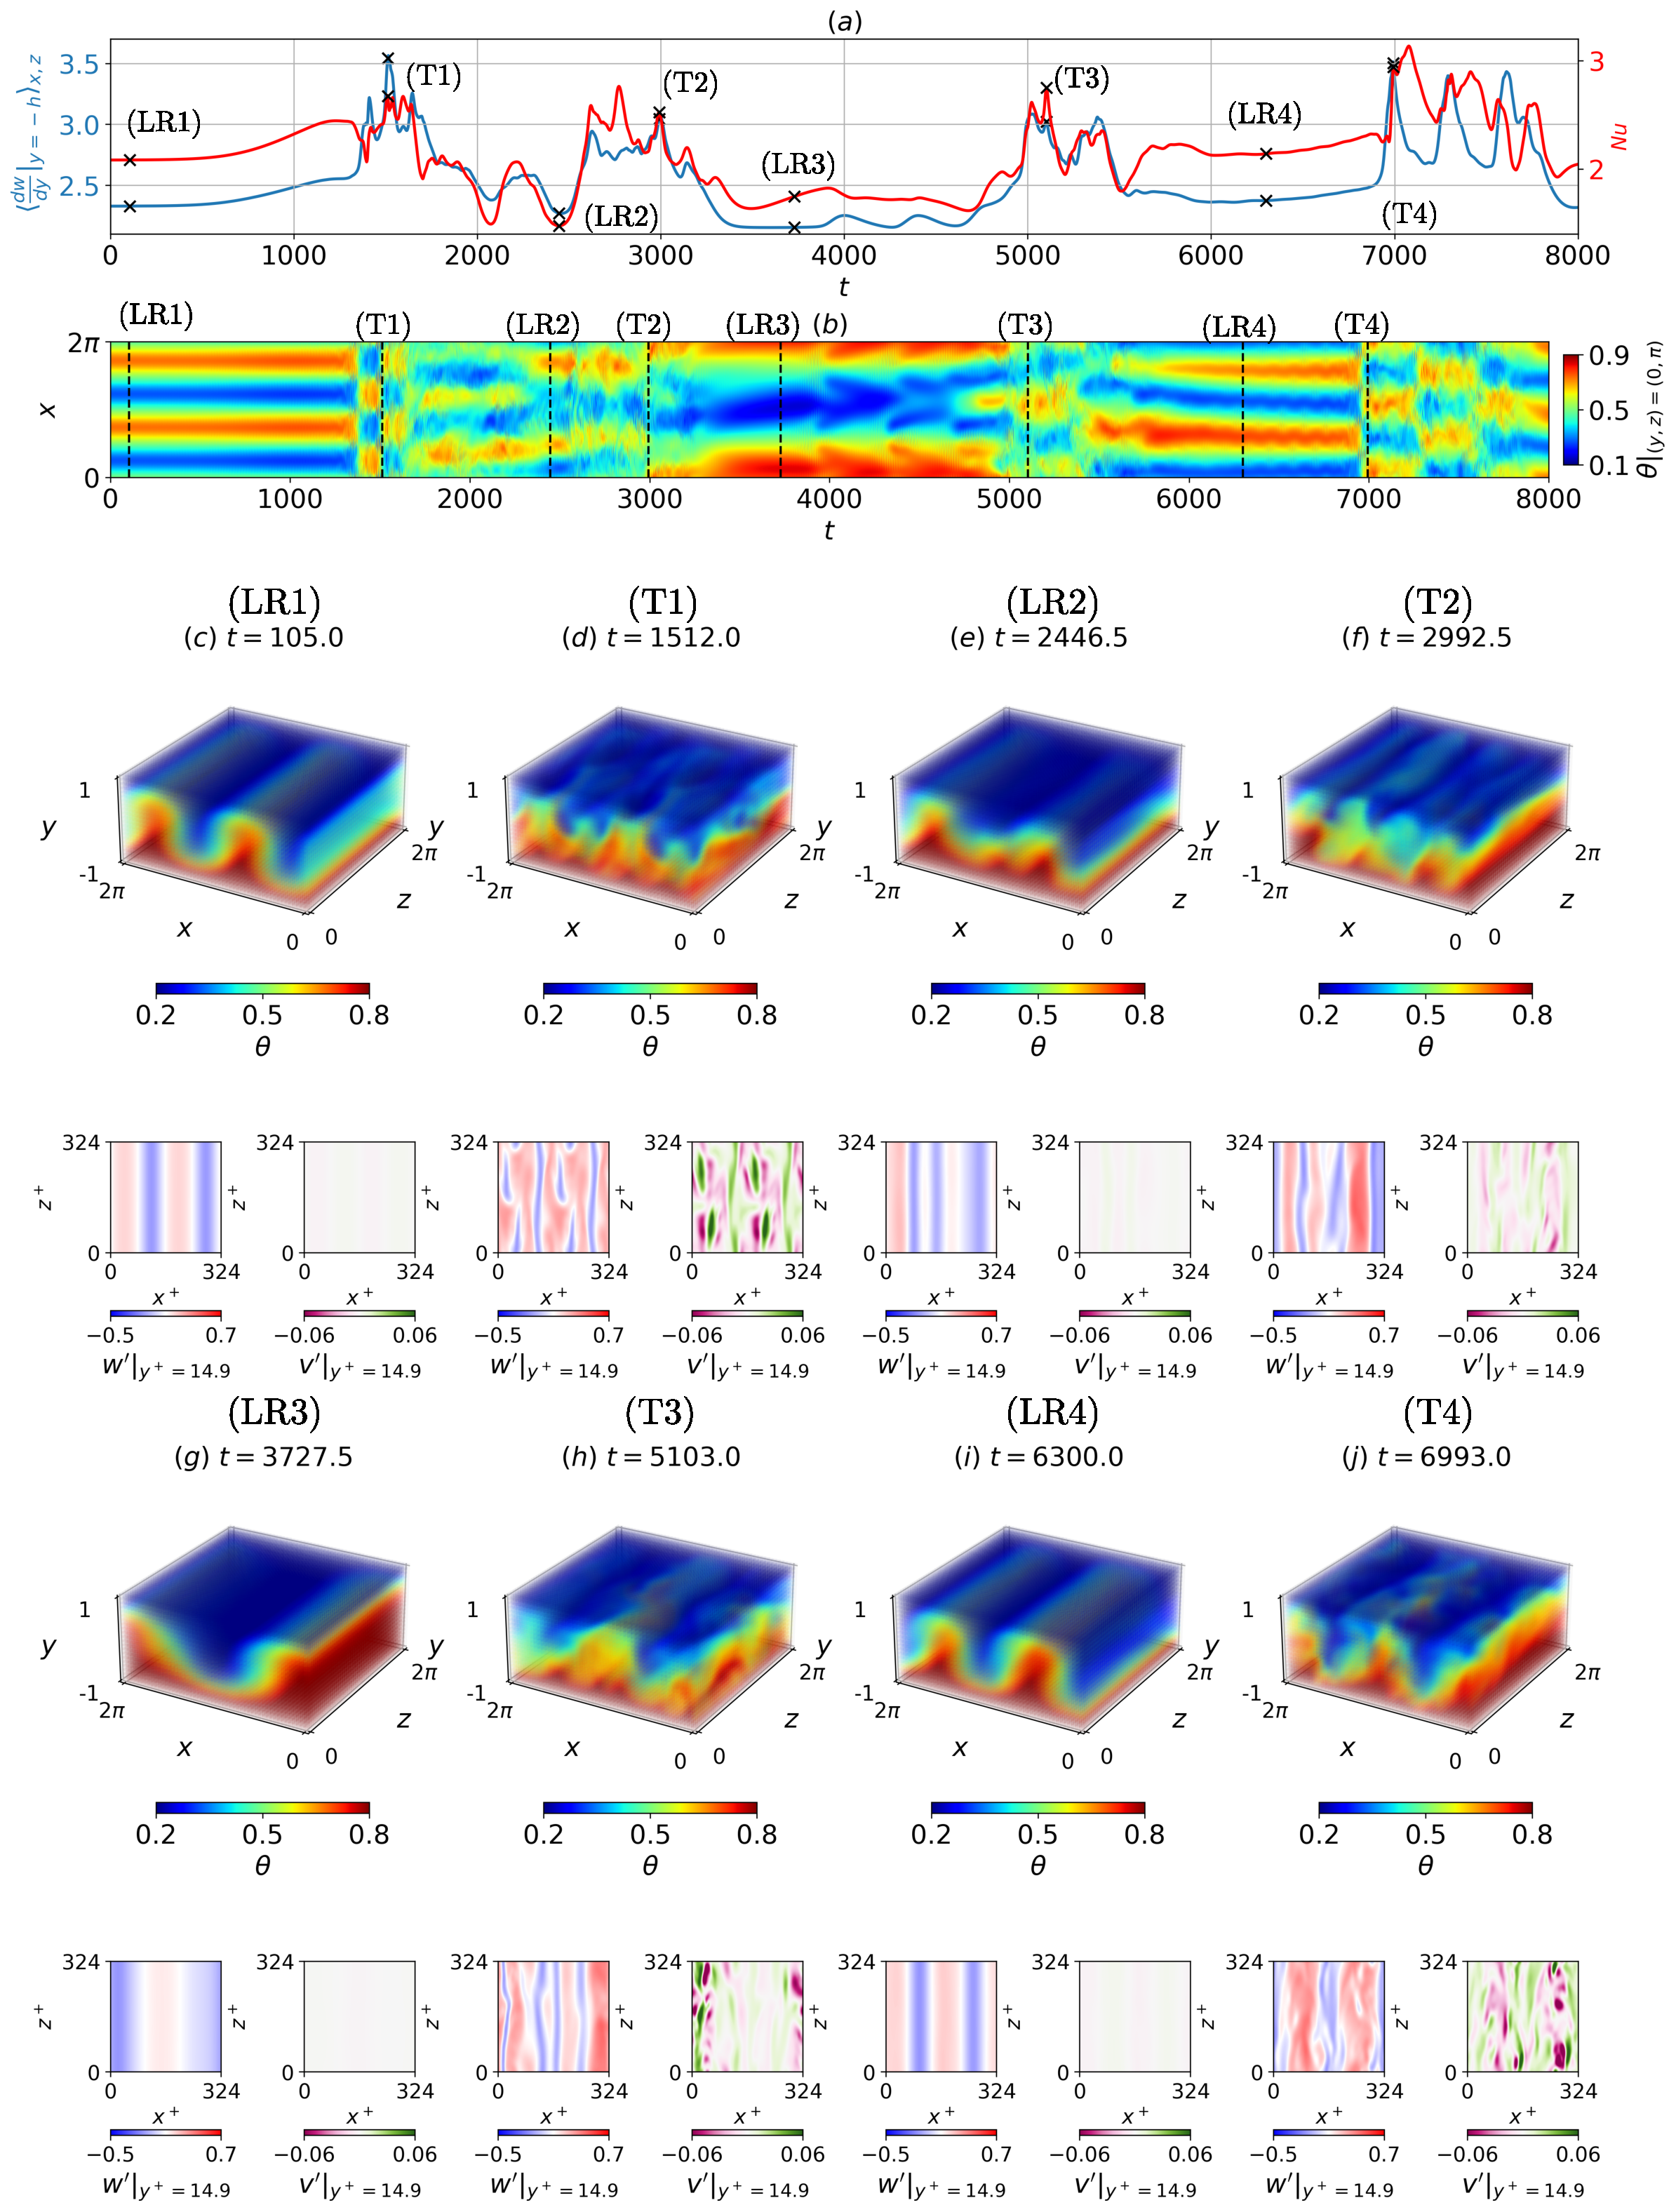
\includegraphics[width=\linewidth]{TransitionalRBP/Figures/RaEffectOnTurbulence/Ra5000-Re1050-MidBotTimeHist-PEig-labelled.pdf}
    \caption{Integrating along the dominant unstable manifold, $\beta d =2$, of the longitudinal rolls at $Ra = 5000, Re = 1050, \Gamma = \pi/2$, $t\in[0,8000]$. Time history of the (a) Nusselt number and shear, and (b) midplane temperature spacetime plot. This system oscillates between the longitudinal rolls ($LR1-4$) and turbulence ($T1-4$) over four intervals. Snapshots of volumetric temperature and near-wall streamwise and spanwise velocity perturbations at (b) $t = 105$, (c) $t = 1512$, (d) $t = 2446.5$, (e) $t = 2992.5$, (f) $t = 3727.5$, (g) $t = 5103$, (h) $t = 6300$, (i) $t = 6993$.}
    \label{fig:intermittent-dynamics}
\end{figure}

Following this, we examine the dominant unstable manifold ($\beta d = 2$) of the longitudinal rolls, by considering an initial condition,
\begin{equation}\label{eq:rbp_SecInstab}
    \mathbf{q}_0(\mathbf{x},t=0) = \mathbf{q}_{LR}(x,y) + \mathbf{\hat{q}}_\beta(x,y)e^{i\beta z},
\end{equation}
which is prescribed to equation \eqref{eq:rbp_RBP}. Here, $\hat{\mathbf{q}}_\beta e^{i\beta d z}$ is an eigenmode at $\beta d$, and the amplitude of which was scaled such that its total energy is defined by,
\begin{equation}\label{eq:rbp_totalenergy}
    \delta = \frac{1}{{V}} \int_\Omega \mathbf{\hat{u}}(\mathbf{x})^T\mathbf{\hat{u}}(\mathbf{x}) + \frac{Ra}{8Re^2Pr}\hat{\theta}(\mathbf{x})^2 \; \mathrm{d}\Omega \approx O(10^{-3})
\end{equation}
is considered.
We have also considered that $\delta = 10^{-2}, 10^{-4}$, where $\delta = 10^{-3}$  was found to be sufficiently small enough to ensure linear growth, while large enough to be computationally practical.

The initial condition is time integrated from $t \in [0, 8000]$, and its time history of near wall transport properties such as the Nusselt number, $Nu$ and shear, $\langle \mathrm{d}w/\mathrm{d}y|_{y=-h}\rangle_{x,z}$, midplane temperature spacetime plot, $\theta|_{(y,z)=(0,\pi)}$, volumetric temperature, $\theta(\mathbf{x})$, and near-wall streamwise and spanwise perturbation velocities snapshots, $w'|_{y^+= 15}, v'|_{y^+=15}$, are presented in figure \ref{fig:intermittent-dynamics}.
% To investigate whether the transition mechanism towards turbulence is due to this linear instability, we consider a numerical experiment along the dominant unstable manifold ($\beta d = 2$) of longitudinal rolls ($\alpha d = 4$).
% The initial condition consists of the dominant secondary eigenmode ($\beta d = 1$), superimposed by longitudinal rolls with streamwise wavenumber, $\alpha d =4$, at $Ra = 5000, Re= 1050$.
% Marked by several `quiescent' and large spikes in the $Nu$ and shear, the solution trajectory visits the longitudinal roll and turbulent states four times, shown as snapshots, labelled $LR1$ to $LR4$, and $T1$ to $T4$ respectively.
The intermittent trajectory is visually present, oscillating between the longitudinal rolls and transient turbulence over four cycles $t = [0, 8000]$, marked by regions of low and high near-wall transport quantities in figure \ref{fig:intermittent-dynamics}(a) and alternating between organised and disorganised longitudinal rolls in figure \ref{fig:intermittent-dynamics}(b).
The snapshots of figure \ref{fig:intermittent-dynamics} illustrate the volumetric temperature field, planar near-wall streamwise and wall-normal perturbations, resembling the longitudinal rolls ($LR1-4$), and transient turbulent states ($T1-4$).
As the solution emerges from the unstable manifold of the longitudinal roll state, $(LR1)$ in figure \ref{fig:intermittent-dynamics}(c), the trajectory erupts into turbulence at $t = 1512$, marked by a disordered volumetric temperature field with high- and low-speed streaks in snapshot $(T1)$ in figure \ref{fig:intermittent-dynamics}(c).
These high- and low-speed streaks are negatively spatially-correlated with wall-normal perturbation velocities in figure \ref{fig:intermittent-dynamics}(d), reminiscent of sweeps and ejection events commonly found in turbulent shear flows \citep{Wallace_1972, Willmarth_1972}.
Notably, the flow structures in snapshot $T1$ in figure \ref{fig:intermittent-dynamics}(d), appear visibly symmetric along the centerline of the channel, $x^+ \approx 162$ (where $x^+= u_\tau x/\nu$ refers to the non-dimensionalised spanwise coordinate), comparable to the invariant states identified in transition shear flows \citep{Waleffe_2001,kerswell2005,eckhardt2007,gibson2008,graham21}.
Turbulence occurs transiently, and the solution decays towards a longitudinal roll-liked state at $t = 2446.5$, shown by snapshot $(LR2)$ in figure \ref{fig:intermittent-dynamics}(e), thereby completing one single cycle.
We note that the snapshot $(LR2)$ does not strictly resemble the longitudinal roll state at snapshot $(LR1)$, however, we show that they are similar and reside close by in state space, as we shall see later.
The intermittent cycle repeats over three subsequent intervals, where the turbulent dynamics and longitudinal rolls emerge at $t = 2992.5, 5103, 6993$, and $t = 3727.5, 6300$, represented as snapshots $(T2,3,4)$ and $(LR3,4)$ in figures \ref{fig:intermittent-dynamics}(f,h,j) and \ref{fig:intermittent-dynamics}(g,i) respectively.

Here, we showed that the dominant unstable manifold of the longitudinal rolls is linked to turbulent dynamics, a transition mechanism based on linear instability.
Interestingly, a `single' longitudinal roll with $\alpha d = 2$ emerges after turbulence decays, shown as snapshot $(LR3)$.
This suggests that other unstable manifolds may be linked to the transition to transient turbulence.

\begin{figure}
    \centering
    \includegraphics[width=\linewidth]{TransitionalRBP/Figures/RaEffectOnTurbulence/Ra5000-Re1050-StateSpace-dudy.png}
    \caption{State space projection based on the planar averaged centerline velocity and shear, coloured by the volume normalised perturbation kinetic energy at $Ra = 5000$, $Re = 1050$, $\Gamma = \pi/2$, (a) $t \in[0,800]$, (b) $t \in [0, 68750]$.  The open black circles represent the unstable equilibria of longitudinal rolls and the laminar state. Note that the black-crosses, labelled by (T1-4) and (LR1-4), refer to temporal snapshots in figure \ref{fig:intermittent-dynamics}, not equilibria solutions.}
    \label{fig:intermittent-state-space}
\end{figure}

To visualise the temporal dynamics in figure \ref{fig:intermittent-dynamics} with better clarity, we project the solution trajectory onto state observables using the planar averaged centerline velocity, $\langle w|_{y=0} \rangle _{x,z}$, shear, $\langle \mathrm{d}w/\mathrm{d}y|_{y=-h}\rangle_{x,z}$ coloured by the volume normalised perturbation kinetic energy, $1/(2V)||\mathbf{u}'||^2$ , in figure \ref{fig:intermittent-state-space}.
These observables seek to distinguish the region of turbulent dynamics, longitudinal roll state, and laminar state residing in near $(0.82, 3.2)$, $(0.90, 2.32)$ and $(1, 2)$, respectively.
This separation is further supported by the location of the temporal snapshots between $(T1-4)$ and $(LR1-4)$, organised near the turbulent dynamics and in longitudinal roll state, $\mathbf{q}_{LR, \alpha d = 4}$, setting them apart.
% Notably, the turbulent dynamics are located near the top left corner, while the longitudinal roll and laminar states are situated at the bottom right corner.
We emphasise that the unstable longitudinal roll state, $\mathbf{q}_{LR, \alpha d = 4}$, and laminar states denoted by open circles are unstable equilibria, while the snapshots longitudinal roll, $(LR1-4)$, and turbulent snapshots, $(T1-4)$, denoted by black crosses, are not.

The solution trajectory emerges from the unstable manifold of the longitudinal rolls, $\mathbf{q}_{LR_{\alpha d = 4}}$, evolving towards turbulent dynamics around $(0.85,3.2)$, denoted by high shear.
Turbulence is transient, occurring with a finite lifetime \citep{hof_2006,schneider_2007}, eventually decaying towards the laminar state.
As the solution trajectory approaches the laminar solution $(1,2)$, it abruptly reverses towards the longitudinal roll state near $(0.95, 2.15)$, $(LR3)$.
Subsequently, the solution trajectory could depart along the unstable manifold of the longitudinal rolls again, leading to the onset of turbulence, where the cycle repeats.

To determine if this cycle could be sustained indefinitely, we consider a longer time horizon, $t \in [0, 68750]$, illustrated in figure \ref{fig:intermittent-state-space}(b).
The solution trajectory wanders between the `cloud' of chaotic transient turbulence at the top left corner (in red), and longitudinal roll and laminar state (in blue) in the bottom right, forming a basin of attraction between the unstable longitudinal rolls, transient turbulence and the laminar state.
We suggest that this basin of attraction, is likely established above a critical $Ra$ as the longitudinal rolls become linearly unstable (i.e $Ra \gtrsim Ra_{s} \approx 4720$, see figure \ref{fig:SecStabLongRolls}(b)), providing an intermediate pathway towards transient turbulence, which could be regenerated again - a `self-sustaining' dynamical process.
We refer to this sustaining process as the \emph{thermally-assisted sustaining process (TASP)}, inspired by the self-sustaining process (SSP) from turbulent shear flows \citep{hkw_1995}.

% The turbulence dynamics near the top left corner are reminiscent of a chaotic saddle in state space \citep{Kreilos_2012, zammert_2015}, where turbulence ultimately relaminarises.
% Over a longer period, the solution trajectory wanders between the `cloud' of turbulent dynamics near (0.85, 0.0035) and the longitudinal rolls near (0.95, 0.0015), distinguished by regions of high and low shear, highlighted as red and blue trajectories.
% We note that in several instances, as the solution trajectory approaches the laminar solution, it `u-turns' abruptly to either $\mathbf{q}_{LR,\alpha d = 2,4}$
% The trajectory emerges from the unstable manifold of the longitudinal rolls, erupting into finite lifetime turbulence which subsequently decays towards the laminar state, which quickly re-energises to the longitudinal rolls, forming a basin of attraction.
% Indeed, the solution trajectory oscillates between the turbulent chaotic saddle, laminar and longitudinal roll state continuously over a longer time horizon, $t \in [0, 68750]$, demonstrating this basin of attraction shown in figure \ref{fig:intermittent-state-space}(b).
% Perhaps this process can be extended to the intermittent regime, where the turbulent chaotic saddle disappears as $Re$ decreases towards $Re = 500$ (see figure \ref{fig:rarephase}), and a cycle between the longitudinal rolls and the laminar state remains, a characteristic of the intermittent role regime in figure \ref{fig:Ra8k-Re500-IntRolls}.
% As $Re$ increases past a threshold $Re$, turbulence is likely to be sustained, where the chaotic saddle stabilises into a chaotic attractor.
% In this case, the solution trajectories are likely to be confined to the chaotic attractor, without ever visiting the longitudinal rolls, and the statistics described by the chaotic attractor defined by $Re$ as in figure \ref{fig:sheardrivenstatistics} suggest.

\subsection{Variation of $Ra$ and $Re$ on the thermally sustained turbulent process within $\Gamma = \pi/ 2$}\label{sec:IntConfined}
\begin{figure}
    \centering
    \includegraphics[width=\linewidth]{TransitionalRBP/Figures/RaEffectOnTurbulence/ConsolidatedPlot-temporal.pdf}
    \caption{The behaviour of the unstable and stable longitudinal rolls at $Ra = 8000, 4000$ for (a,e) $Re = 600$, (b,f) $Re = 700$, (c,g) $Re = 1000$ and (d,h) $Re = 1400$ within $\Gamma = \pi/2$. Each parameter regime consist of three panels from the top to bottom, depicting the midplane temperature spacetime plot, $\theta|_{(y,z) = (0, \pi)}$, time history of the Nusselt number and shear, and state space projection based on the planar averaged centerline velocity and shear, coloured by the volume normalised perturbation kinetic energy.}
    \label{fig:dynamical-process}
\end{figure}
In this section, we explore the behaviour of the \emph{TASP} as $Re$ and $Ra$ are varied.
We consider eight different cases at $Ra = 8000, 4000$ and $Re = 600, 700, 1000, 1400$.
The results of these eight cases, where longitudinals rolls are either unstable at $Ra = 8000$ or stable at $Ra = 4000$, are shown in figure \ref{fig:dynamical-process}, depicting the spacetime plots of midplane temperature, $\theta|_{y=0}(x,t)$, time history of the Nusselt number, $Nu$, and shear, $\langle \mathrm{d}w/\mathrm{d}y|_{y=-h}\rangle_{x,z}$ and state space projection using the planar averaged centerline velocity, $\langle w|_{y=0} \rangle_{x,z}$, shear, coloured by the volume normalised perturbation kinetic energy, $\frac{1}{2V}||\mathbf{u'}||^2$.
For all cases except $Ra = 4000$, $Re = 1000$ and $Re = 1400$, their initial conditions are prepared from the laminar state, superimposed by a random noise based on a Gaussian distribution with zero mean and unit variance, scaled to a total energy of $\delta = 10^{-3}$ (see definition in equation \eqref{eq:rbp_totalenergy}).
For the exceptional cases at $Ra = 4000$, $Re = 1000$ and $Re = 1400$, where subcritical turbulence and stable longitudinal rolls are expected, their initial conditions are obtained by gradually lowering $Re$ from a statistically stationary turbulent solution at $Re = 2000$.
We note that we have not explicitly performed a linear stability analysis of the longitudinal rolls for the parameter regime in figure \ref{fig:dynamical-process}, however, they appear to be unstable at $Ra = 8000$, while being stable at $Ra = 4000$ from DNS.

At $Ra = 8000$, $Re = 1000$, $t \in [0, 10000]$ in figure \ref{fig:dynamical-process}(c), the trajectory visits the transient turbulent regime near $t=7200$, which decays towards the longitudinal roll state, $\mathbf{q}_{LR}$, at $t = 7400$, which could be regenerated again, consistent with the \emph{TASP} in \S \ref{sec:TASP}.
% As $Ra$ decreases to $4000$, the longitudinal rolls become linearly stable, emerging as an asymptotically stable state.
% To illustrate this, the initial condition at $Ra = 4000, Re = 1100$ (gradually lowered from $Re=2000$) is time-integrated for $t = [0, 1500]$ in figure \ref{fig:dynamical-process}(g).
% \To illustrate this case in figure \ref{fig:dynamical-process}(g), where the initial condition is taken from a statistically stationary turbulent state at $Re = 2000$, and then gradually lowered to $Re = 1100$.
% As $Ra$ is lowered to $4000$, the basin of attraction disappears in figure \ref{fig:dynamical-process}(g).
As $Ra$ is lowered to $4000$, the solution trajectory decays towards the longitudinal roll state, $\mathbf{q}_{LR}$, where the \emph{TASP} disappears.
In this case, the longitudinal rolls are linearly stable, confirming our hypothesis earlier that the \emph{TASP} is only established when longitudinal rolls become linearly unstable above a certain $Ra$-threshold (i.e $Ra \gtrsim Ra_{s} \approx 4720$).
% This confirms our hypothesis earlier, that the \emph{thermally-assisted sustaining process} is only established above a certain $Ra$-threshold, i.e. $Ra \gtrsim Ra_{s} \approx 4720$.
% Figures \ref{fig:dynamical-process}(c,g) demonstrate the nature of transient turbulence at $Re = 1100$.
% As turbulence is transient, the solution trajectories decay towards the laminar state at $Ra = 4000$, whereas at $Ra = 8000$, it becomes re-energised via unstable longitudinal rolls, forming the \emph{thermally sustained turbulent process}.

% As $Re$ increased from $1000$ to $1400$, turbulence is likely to be sustained shown in figures \ref{fig:dynamical-process}(d,h).
At $Re = 1400$, $Ra = 4000$, the solution trajectory remains within the turbulent `cloud' near $(0.8, 3.8)$ illustrated in figure \ref{fig:dynamical-process}(h), suggesting that turbulence might be sustained indefinitely, in which the turbulent chaotic saddle at $Re = 1000$ could be transformed into a chaotic attractor at $Re = 1400$.
% The longitudinal rolls are linearly stable here, leading to a bistable system where both turbulence and the stable longitudinal rolls can coexist as bistable attractors, analogous to subcritical turbulence.
As $Ra$ is increased to $8000$, the solution trajectory originating from the laminar state, evolves towards the unstable longitudinal roll state, $\mathbf{q}_{LR}$ at $t = 1550$, transitioning into sustained turbulence at $t= 1800$.
Therefore, the linearly unstable longitudinal rolls serve as an intermediate transitional pathway between the laminar state and subcritical turbulence, whereas at $Ra = 4000$, a bistability between stable longitudinal rolls (not shown) and turbulence is established.
% However, a key difference lies in the transition pathway from the laminar state to turbulence.
% At $Ra = 8000$, the initial condition is integrated for $t = [0, 10000]$.
% Starting from the laminar state, the solution trajectory evolves towards the longitudinal roll state, $\mathbf{q}_{LR}$ at $t = 1550$, and subsequently along its unstable manifold, erupting into turbulence at $t = 1800$ where the solution trajectory remains confined in the attractor.
% This demonstrates an indirect transition pathway from the laminar state towards turbulence via an unstable longitudinal roll state.

Next, we examine the behaviour of \emph{TASP} as $Re$ decreases towards the intermittent regime at $Re = 600, 700$, where a periodic orbit emerges between the longitudinal roll and the laminar state.
At $Re = 600, Ra = 8000$ in figure \ref{fig:dynamical-process}(a), the solution trajectory initially evolves towards the longitudinal roll state, $\mathbf{q}_{LR}$, which is linearly unstable and breaks down towards the laminar state at $t = 2200$.
This breakdown is evidenced by the trajectory's proximity to the laminar state in state space and the presence of a narrow green patch in the midplane temperature spacetime plot.
The longitudinal roll state is regenerated again, forming a periodic orbit with a period of $T_{period} = 8098-6108 =1990$, oscillating between the longitudinal roll and laminar state over five intervals within $t \in [0, 10000]$.
As $Re$ increases slightly to $700$, the periodic orbit persists over a shorter period of $T_{period} = 3889 - 3386 = 503$.
A notable difference is observed in the regenerated longitudinal rolls, which is continuously translated by $L_x/2$ in the $x$-direction.
Additionally, as $Re$ increases from $600$ to $700$, the trajectory moves further away from the laminar state during breakdown, suggesting an increasing attraction towards the longitudinal roll state, $\mathbf{q}_{LR}$ (compare $t = 2200$ in figure \ref{fig:dynamical-process}(a) and $t = 2750$ in figure \ref{fig:dynamical-process}(b)).
When $Ra$ is lowered to $Ra = 4000$, the periodic orbit disappears and the trajectory stabilises into the longitudinal roll state, $\mathbf{q}_{LR}$, at $Re = 600, 700$.
% At $Re = 600$, $Ra = 8000$ in figure \ref{fig:dynamical-process}(a), the solution evolves towards the longitudinal roll state, $\mathbf{q}_{LR}$, from the laminar solution.
% Nonetheless, a periodic orbit is established at $Ra = 8000$, $Re = 600,700$, likely connecting between the laminar state and the longitudinal roll state.
% Although the conditions in terms of $Ra$ and $Re$ considered here differ from figure \ref{fig:SecStabLongRolls}, the critical $Ra_{s} \approx 4720$ identified earlier supports our findings here, highlighting the role of $Ra$ in sustaining turbulence via unstable longitudinal rolls.
\begin{figure}
    \centering
    \includegraphics[width=\linewidth]{TransitionalRBP/Figures/RaEffectOnTurbulence/statespace-cartoon-full.pdf}
    \caption{A state space sketch of figure \ref{fig:dynamical-process} at $Ra = 8000$, (a) $Re = 600$, (b) $Re = 700$, (c) $Re = 1000$, (d) $Re = 1400$ and $Ra = 4000$ at (e) $Re = 600,700$, (f) $Re = 1000$, (g) $Re =1400$. The longitudinal roll is linearly unstable (saddle) at $Ra = 8000$, and is stable at $Ra = 4000$, whereas the laminar state is always linearly unstable (saddle). The blue and orange solid arrows refer to the unstable manifold of longitudinal rolls and the laminar state. The red solid lines denote the chaotic trajectories of turbulence, likely forming a chaotic saddle at $Re = 1000$ and a chaotic attractor at $Re = 1400$. The black-dashed trajectories refer to possible solution trajectories, forming a periodic orbit (P.O) at $Ra = 8000$, $Re = 600, 700$, and a basin of attraction (B.o.A) at $Ra = 8000, Re = 1000$. We note that invariant states could exist at $Ra = 4000, Re = 600,700$, labelled as a saddle here \citep{Paranjape_2023}.}
    \label{fig:statespacesketch}
\end{figure}

To summarise the dynamical processes identified in figure \ref{fig:dynamical-process}, we present a state space sketch of it in figure \ref{fig:statespacesketch}.
At $Ra = 8000$, $Re = 600$ and $Re= 700$, the longitudinal rolls become linearly unstable, breaking down into the laminar state before being regenerated, forming a periodic orbit illustrated enclosed by black dotted paths in figures \ref{fig:statespacesketch}(a,b).
For $Re = 700$, the regenerated longitudinal roll is continuously translated by $L_x/2$, suggestive a possible merger of two periodic orbits into one sketched in figure \ref{fig:dynamical-process}(b).
Future bifurcation studies are required to establish this, providing an avenue for future work.
% At $Re = 600$ and $Re = 700$, turbulence does not appear to exist as it is far below the threshold for the onset of turbulence near $Re \sim 1000$ (see figure \ref{fig:rarephase} references in \S \ref{sec:PPF}).
% We emphasise that we are not certain that if the unstable manifold of the longitudinal rolls are linked to the stable manifold of the laminar state, hence, the orange arrow is shifted away from the stable manifold of the laminar state.
% The key difference between $Re = 600$ and $ Re = 700$ may lie in the proximity of the periodic orbit with the laminar state as highlighted between figure \ref{fig:dynamical-process}(a) and \ref{fig:dynamical-process}(b).
% As $Re$ increases, the solution trajectory moves further away from the laminar state, becoming more strongly attracted towards the longitudinal roll state.
As $Ra$ is lowered to $Ra = 4000$, the laminar state stabilises into the longitudinal rolls in figure \ref{fig:statespacesketch}(e).
This regime may contain invariant solutions \citep{Paranjape_2023}, denoted as saddle points here.
Integrating along the unstable manifold of longitudinal rolls at $Ra= 8000, Re = 1000$ leads to transient turbulence, which eventually decays to the laminar state before regenerating into longitudinal rolls again, forming the \emph{TASP} in figure \ref{fig:statespacesketch}(c).
In contrast, at $Ra = 4000, Re = 1000$, the longitudinal rolls become linearly stable, eliminating the intermediate (orange) pathway toward turbulence where transient turbulence stabilises into longitudinal rolls shown as the black-dashed trajectory in figure \ref{fig:statespacesketch}(f).
For $Ra = 8000, Re = 1400$, the linearly unstable longitudinal rolls provide an intermediate pathway towards turbulence from the laminar state sketched in figure \ref{fig:statespacesketch}(d), breaking the bistability between the laminar state and subcritical turbulence seen at $Ra = 4000$ in figure \ref{fig:statespacesketch}(g).
This behaviour resembles the nature of subcritical turbulence in shear-driven flow, highlighting the contribution of unstable longitudinal rolls towards the transition to turbulence within $\Gamma = \pi/2$.

We examined the dynamics of unstable longitudinal rolls as the Reynolds number, $Re$, and Rayleigh number, $Ra$, are varied, identifying three key dynamical processes: (1) periodic orbits between longitudinal rolls and the laminar state (figure \ref{fig:statespacesketch}(a,b)), (2) the \emph{TASP}, where transient turbulence can be sustained (figure \ref{fig:statespacesketch}(c)) and (3) an intermediate transitional pathway towards sustained turbulence (figure \ref{fig:statespacesketch}(d)).
To establish a connection between these processes and understand their transitional boundaries, we conduct a parameter sweep over $Ra \in [4000, 10000]$ and $Re \in [600, 1400]$ within $\Gamma = \pi/2$.
Figure \ref{fig:compiled-full} presents the midplane temperature spacetime plot alongside the time history of shear, $\langle \mathrm{d}w/\mathrm{d}y|_{y=-h}\rangle_{x,z}$ and the Nusselt number, $Nu$.
For all simulations, the initial conditions are prepared from the laminar state, superimposed with a random noise based on a Gaussian distribution with zero mean and unit variance, scaled to a total energy of $\delta = 10^{-3}$ (see definition in equation \eqref{eq:rbp_totalenergy}).
Due to the subcritical nature of turbulence and expected stable longitudinal rolls, exceptions are made for $Ra = 4000$, $Re \in [900, 1400]$, where initial conditions are taken from gradually lowering $Re$ from a statistically stationary turbulent state at $Re = 2000$.
The \emph{thermally-assisted sustaining process} is highlighted in green for $Ra \in [5000, 10000]$ and $Re \in[900, 1200]$, where temporally intermittent shear and Nusselt number fluctuations are observed, accompanied by a mixture of organised and disorganised flow structures in the temperature spacetime plots.
In this regime, the longitudinal rolls provide an intermediate pathway towards transient turbulence, which appears linearly unstable for $Ra \geq 5000$.
Below this threshold, transient turbulence decays into stable longitudinal rolls, as observed at $Ra = 4000$, $Re \in [900, 1200]$ labelled as 'transient turbulence'.
Periodic orbits between longitudinal rolls and the laminar state occur for $Ra \in [6000, 10000]$ and $Re \in [600,800]$, establishing above a critical $Ra-Re$ threshold, below which solutions stabilise into longitudinal rolls shaded in red.
Notably at $Re = 800$, the periodic orbit becomes increasingly quasi-periodic, likely related to the \emph{TASP} near $Re \sim 900$.
Despite longitudinal rolls being linearly stable at $Ra = 4000, Re = 1400$ (not shown), turbulence is sustained, shaded in blue across $Re = 1400$.
In this case, a bistable system forms between longitudinal rolls and turbulence at $Ra = 4000$, while the longitudinal rolls provide an intermediate pathway towards turbulence for $Ra \geq 5000$.
Figure \ref{fig:compiled-full} underscores the role of unstable longitudinal rolls in transitional RBP flows within confined domains.

% The three key processes of the \emph{TASP}: (1) quasi-periodic orbits, (2) sustained transient turbulence, and (3) sustained turbulence are evident beyond a $Ra-Re$ boundary, below which longitudinal rolls remain asymptotically stable.
% At $Re = 1400$, turbulence is sustained, with the chaotic saddle likely transforming into a chaotic attractor.
% On the other hand, at $Ra = 4000$, a bistable system between longitudinal rolls and the turbulent attractor emerges, represented by two separate black-dashed solution trajectories in figure \ref{fig:statespacesketch}(g).


\begin{figure}
    \centering
    \includegraphics[width=1.47\linewidth, angle=90]{TransitionalRBP/Figures/RaEffectOnTurbulence/ConsolidatedPlot-full-annotated.pdf}
    \caption{The temperature spacetime plots and time history of shear and the Nusselt number for $Ra \in [5000, 10000]$, $Re \in [600, 1400]$ within $\Gamma = \pi/2$. Unstable longitudinal rolls lead to the onset of (1) periodic orbits (yellow), (2) the \emph{thermally-assisted sustaining process} (green), and (3) sustained turbulence (blue), occurring beyond an $Ra-Re$ boundary, below which longitudinal rolls remain stable (red).}
    \label{fig:compiled-full}
\end{figure}

\subsection{Extending to large domains, $\Gamma = 4\pi$.}
\begin{figure}
    \centering
    \includegraphics[width=\linewidth]{TransitionalRBP/Figures/RaEffectOnTurbulence/Ra10000-MidSpaceTimeAndPDFs.pdf}
    \caption{The midplane temperature spacetime plot, and near-wall wall-normal and spanwise perturbation kinetic energy by normalised by thermal velocity scale, $u_\kappa$, and the probability density functions based on planar-averaged centerline velocity and the midplane temperature at $Ra = 10000$, (a,b,c) $Re = 500$, (d,e,f) $Re = 750$, (g,h,i) $Re = 1000$, (j,k,l) $Re = 1050$.}
    \label{fig:Ra10k-PDFs}
\end{figure}

In this section, we bridge the gap between the confined and large domains by discussing the relevance of dynamical processes within the confined domains to the large domains, $\Gamma = 4\pi$.
We will focus on the intermittent roll and shear-driven turbulence regime at $Ra = 500, 750, 1000, 1050$ for $Ra = 10000$ presented by figure \ref{fig:Ra10k-PDFs}, illustrating their spacetime plots of midplane temperature, $\theta|_{(y,z)=(0,8\pi)}$, and near-wall wall-normal and spanwise perturbation kinetic energy, $\mathcal{E}_{u'+v'}$.
Additionally, we also examine the probability distribution functions based on the centreline-velocity normalised midplane velocity and temperature, $f(w|_{y=0}, \theta|_{y=0})$.
% Based on the processes summarised in figure \ref{fig:statespacesketch}, we expect three processes: (1) interactions between longitudinal roll and laminar state in the intermittent roll regime at $Re = 500, 750$, (2) the \emph{TASP} and (3) an intermediate transitional pathway where turbulence is sutained at $Re = 1000, 1050$ within $\Gamma = 4\pi$.
At $Ra = 10000$, $Re = 500$, the breakdown of longitudinal rolls towards the laminar state is observed, highlighted by spatially-localised green spots in the midplane temperature plots, and dark regions in the near-wall perturbation kinetic energy spacetime plot near $t = 500, 3800$ in figure \ref{fig:Ra10k-PDFs}(a,b) respectively.
As $Re$ increases from $500$ to $750$, the breakdown towards the laminar state remains visually apparent. 
The spatiotemporal dynamics between longitudinal rolls and the laminar state within the intermittent regime in the large domain are reminiscent of the periodic orbit identified between them in a confined domain.
There is a noticeable decrease in the number of green and dark regions between figures \ref{fig:Ra10k-PDFs}(a,b) and (d,e), suggesting fewer laminar events at $Re = 750$.
Indeed, this difference is further reflected in their PDFs, where the probability of laminar events, at $(w|_{y=0}, \theta|_{y=0}) = (1,0)$, depicted as the `head' of the `arc-shaped' PDF decreasing from $Re = 500$ (figure \ref{fig:Ra10k-PDFs}(c)) to $Re = 750$ (figure \ref{fig:Ra10k-PDFs}(f)).
This likely suggests fewer laminar state events and more occurrences of the longitudinal roll state, as the solution trajectory becomes increasingly attracted towards the longitudinal roll state from $Re = 600$ and $Re = 700$ at $Ra= 8000$ in the confined domain presented in figures \ref{fig:dynamical-process}(a,b).
% This observation qualitatively agrees with the behaviour at $Ra = 8000$, $Re = 700$ in figure \ref{fig:dynamical-process}.
% Using the centreline-velocity normalised midplane streamwise velocity as an observable, the solution trajectory retreats from the laminar state during breakdown, becoming increasingly attracted to the longitudinal roll state.

At $Re = 1000$, we observe the coexistence of the laminar state, the longitudinal rolls and transient turbulence appearing as dark, bright and very bright regions in the near-wall wall-normal and spanwise perturbation velocities, normalised by thermal velocity scale, $\mathcal{E}_{u' +v'}/u_\kappa^2$ (where $u_\kappa = \kappa / d$) in figure \ref{fig:Ra10k-PDFs}(h).
Starting at $t = 2000$, the longitudinal rolls appearing as red/blue elongated strips in figure \ref{fig:Ra10k-PDFs}(g) erupt into turbulence at $t = 2500$, appearing as very bright spots in figure \ref{fig:Ra10k-PDFs}(h).
Turbulence is transient, decaying towards the laminar state at $t = 3000$, as indicated by the dark patches in figure \ref{fig:Ra10k-PDFs}(h).
By $t = 4000$, longitudinal rolls are regenerated, appearing as red/blue elongated strips in figure \ref{fig:Ra10k-PDFs}(g).
This process resembles \emph{TASP} in a confined domain (figure \ref{fig:statespacesketch}(c)), suggesting that a similar process may be present in the large domain.

As $Re$ approaches $Re = 1050$, turbulence becomes sustained, forming distinct turbulent-laminar bands as seen in figure \ref{fig:Ra10k-PDFs}(k,h).
The increase in turbulent events is reflected by the PDFs, where a `D'-shaped PDF absent in $Re = 750$, gradually increases in intensity from $Re = 1000$ to $Re = 1050$.
The lack of prolonged laminar spots, previously identified for $Ra = 0$ (figure \ref{fig:spacetime-Ra0k-Re1.05k} suggests that the longitudinal rolls provide an intermediate pathway towards turbulence in a small domain (figure \ref{fig:dynamical-process}(d)).

\section{Conclusions}\label{sec:rbp_5}
We conclude by summarising the key findings of transitional RBP from figure \ref{fig:rarephase}, where we identify five different regimes and their transition boundaries.
First, we examined the bistability between SDC and ISRs in RBP flows, which persists up to $Re = 1$, beyond which only ISR solutions are observed.
The critical $Re_{s}$ at which SDC disappears likely depends on $Re$ and remains an avenue for future study.
At $Re = 10$, the wavenumber of the stable ISRs adheres to the stability boundaries of the Busse balloon, and we observe longitudinal rolls as well as oscillatory longitudinal rolls, expected from the secondary instabilities of RBC \citep{Clever_Busse_1974}.
Wavy rolls appear at $Re = 100$, $Ra \geq 5000$ \citep{Clever_Busse_1991,pabiou_2005}, but disappear for $Re \geq 500$, where a new regime referred to as the intermittent rolls emerges.
This regime is characterised by the spatiotemporal intermittent breakdown of longitudinal rolls towards the laminar state, before being regenerated again.
Similar to the wavy rolls regime, intermittent rolls only appear above a $Ra$-threshold, $Ra \geq 5000$ (see figure \ref{fig:rarephase}), below which longitudinal rolls persists.
Notably, the wavenumber of these longitudinal rolls lies outside of the stability boundaries of the Busse balloon for RBC ($Re = 0$), suggesting the stability boundaries are modified as $Re$ increases, a potential avenue for future work. 
As $Re$ approaches the shear-driven turbulent regime, we observe the coexistence of longitudinal rolls with neighbouring turbulent bands at $Ra = 10000$, highlighting the role of the spatiotemporal nature of longitudinal rolls in transitional RBP.

To investigate the role of longitudinal rolls in transitional RBP, we consider a confined domain, $\Gamma = \pi/2$, where spatial intermittency can be artificially suppressed.
Integrating along the unstable manifold of longitudinal rolls in the confined domain leads to transient turbulence, which eventually decays towards the laminar state before longitudinal rolls re-emerge again.
Transient turbulence can be sustained here, referred to as the \emph{thermally-assisted sustaining process (TASP).}
To understand \emph{TASP} further, we explore its behaviour as $Re$ and $Ra$ are varied.
As $Re$ decreases towards the intermittent rolls regime, a periodic orbit emerges, oscillating between the longitudinal roll and a laminar state.
In contrast, as $Re$ increases, shear-driven turbulence becomes sustained, with the longitudinal rolls providing an intermediate route towards the transition to turbulence from the laminar state.
Our investigation of the role of unstable longitudinal rolls within confined domains revealed three dynamical processes: the onset of (1)periodic orbits, (2) the \emph{TASP}, and (3) providing an intermediate route towards turbulence.
It was also shown that the stability of longitudinal rolls largely depends on $Re$ and $Ra$, below which only stable longitudinal rolls are observed.
Furthermore, the connection between the dynamical process identified here to the onset of wavy rolls warrants further investigation.
We also acknowledge that more spatially subharmonic instabilities may arise as the domain size increases.

Finally, we assess the relevance of our findings in the confined domain and their connection to the large domain.
We suggest that the breakdown towards the laminar state in the intermittent roll regime bears qualitative similarities to the periodic orbit between them in the confined domain.
Furthermore, transient turbulence that is sustained by longitudinal rolls is also evident in the large domain, where the flow transitions between transient turbulence, longitudinal rolls and the laminar state in figures \ref{fig:Ra10k-PDFs}(g,h).
At $Re = 1050$, the turbulent-laminar bands dominate, weakly dependent on $Ra$, as suggested by figure \ref{fig:sheardrivenstatistics}.
It may be possible that these turbulent-laminar bands decay spontaneously towards the laminar state \citep{tuckerman_2014,Gome_2020}, and their lifetime statistics may depend on $Ra$, which warrants further investigation.
However, if the \emph{TASP} persists above a critical $Ra$ providing a pathway to turbulence, then the turbulent-laminar bands could be sustained indefinitely.
As $Re$ approaches $2000$, featureless turbulence emerges, with the first- and second-order statistics becoming independent of $Re$, indicating fully developed turbulence. 
It is likely that the range of $Ra \in [0, 10000]$ considered here is too low to significantly influence shear-driven turbulence at $Re = 2000$, suggested by the studies of turbulent RBP \citep{pirozzoli_2017}.

% The influence of $Re$ on the stability boundaries of the Busse balloon is not studied, which warrants further investigation.
% The first and second statistics of the states encompassing the buoyancy-dominated regime are compared, and their similarity indicates that the underlying physical mechanism is described by the buoyancy-driven Rayleigh-B\'{e}nard convection, and is only weakly dependent on $Re$.
% the relevance of our findings in the MFU and its connection to the large domain, $\Gamma = 4\pi$.
% We suggest that the intermittent roll states are closely linked to the periodic orbit between longitudinal rolls and the laminar flow within the MFU at $Re = 600, 700$, $Ra = 8000$.
% At $Re = 1000$, we encounter a regime where the laminar state, transient turbulence and longitudinal rolls could coexist, indicative of the \emph{thermally sustained turbulent process} identified earlier within an MFU.

% This process was then analysed by linear stability analysis of the longitudinal rolls, whereby integrating along the unstable manifold of longitudinal rolls led to transient turbulence, eventually decaying towards the laminar state before re-energising into longitudinal rolls again, forming a basin of attraction.
% This basin of attraction is also found to occur at $Ra = 8000$, $Re = 1100$, but not $Ra = 4000$, suggesting that the pathway towards transient turbulence is removed when the longitudinal roll become linearly stable below a certain $Ra$ threshold - possibly related to the critical $Ra_s = 4720$ in figure \ref{fig:SecStabLongRolls}.
%As $Re$ is lowered further to $Re = 600$, the transient turbulent regime ceases to exist, where the solution trajectories form a periodic orbit, oscillating between the laminar solution and the longitudinal roll state at $Ra = 8000$, but not at $Ra = 4000$ where the longitudinal rolls become asymptotically stable.
% It  be possible to envisage that this periodic orbit could consist of heteroclinic orbits between the unstable longitudinal rolls and unstable wavy rolls, or the laminar state.
% However, this remains as a potential future work.
% As $Re$ increases to $1600$, shear-driven turbulence is sustained, likely emerging as a chaotic attractor above a certain $Re$ threshold.
% As such, the unstable longitudinal rolls provide an alternative pathway for the transition from the laminar state towards subcritical turbulence.
% The dynamics within the MFU are briefly summarised in figure \ref{fig:statespacesketch}.

% \begin{enumerate}
%     \item Is the unstable manifold of the longitudinal roll connected to the laminar state? 
%     \item How does subcritical $Ra$ enhance turbulence as we have seen.
%     \item How does wavy rolls transition to intermittent roles and what is the physical mehcnaism?
% \end{enumerate}

% Next, we propose that the impact of the thermally sustained turbulent process may extend to the intermittent rolls regime for $Ra \geq 5000$ and $Re \in [500, 1000]$.
% As the intermittent rolls behave as the dominant structure within this regime, it `bursts spontaneously before re-energizing as an intermittent roll once again, this is reminiscent of the thermally sustained turbulent process in a special case where the turbulent chaotic saddle appears to be small, as the solution trajectory jumps towards the 
% 
% Next, we show the effect of thermally sustained turbulent process for lower $Re$ by using the probability density functions are lower $Re$ in figure.
% The PDF at $Re = 1050$ is shown to have a dense arrowhead shape, while the wavy convection rolls have an arch shape with peaks at two corners, and as $Re$ increases, the head is darkened, likely indicating the presence of weak turbulence.

% For $Ra < Ra_{c,sec}$, the longitudinal rolls become linearly stable, transforming into a stable node and removing the orange pathway towards turbulence, where the longitudinal roll emerges as a stable state within $\Gamma = \pi / 2$.
% This highlights the role of $Ra$ in sustaining turbulence through the linear instability of longitudinal rolls.

% For $Re > 1050$, the chaotic saddle could transform into a chaotic attractor, where turbulence emerges as the basin of attraction, and the intermittent dynamics between longitudinal rolls and turbulence cease to exist

% In this case, we have considered the impact of $Ra$ and $Re$ in isolation, directly impacting the stability of longitudinal rolls, and turbulence independently.

%  However, this may not hold true as raising $Ra$ may alter the nature of the chaotic saddle, turning it into a chaotic attractor which warrants further investigation.
% have assumed that its impact on the nature of the turbulent chaotic saddle remains negligible, which may not hold true.
% As $Ra$ is increased further, the turbulent chaotic saddle may transform into a chaotic attractor, where turbulence is sustained, eliminating the intermittent cycle.
% The impact of $Ra$ on the nature of the chaotic saddle warrants further investigation.

% The mean across $Ra$ is labelled as the `turbulent core' located at which slowly shifts from $(0.935,0.5)$ to $(0.919,0.5)$ as from $Ra = 0$ to $Ra = 10000$, indicating a more blunted turbulent profile expected from figure \ref{fig:Re1050-Ra-Stats}(a).
% As $Ra$ is increased, this localised speck disappears while the turbulent `core' slowly shifts from $(0.935,0.5)$ to $(0.919, 0.5)$ demonstrating the increased in likelihood of turbulent events.
% We suggest that the thermally sustaining turbulent process extends to lower $Re$, i.e the intermittent rolls regime, we observe laminar regions due to the breakdown in turbulent event.
% To demonstrate this increase in likelihood, we present a 2D normalised histogram measured by volume normalised perturbation kinetic energy and normalised stream- and spanwise averaged centreline velocity between $Ra = 0$ and $Ra = 100000$ in figure \ref{fig:Re1050-Ra10k0k-hist}(a,b) respectively.

% At $Ra = 0, Re = 1050$, this mechanism cannot exist, and turbulence is sustained in the form of spatially-intermittent turbulent laminar bands within $\Gamma = 4\pi$ in figure \ref{fig:spacetime-Ra0k-Re1.05k}.
% At $Ra = 10000, Re = 1050$, where the thermally sustained turbulent process is expected within a spatially localised region, turbulence is therefore more likely to exist in $\Gamma = 4\pi$, which might explain the absence of non-turbulent regions in figure \ref{fig:spacetime-Ra10k-Re1.05k}.
% To demonstrate this increase in likelihood, we present a 2D normalised histogram measured by volume normalised perturbation kinetic energy and normalised stream- and spanwise averaged centreline velocity between $Ra = 0$ and $Ra = 100000$ in figure \ref{fig:Re1050-Ra10k0k-hist}(a,b) respectively.
% In the case of $Ra = 0$, the state dynamics wanders between a turbulent, and mildly turbulent state, the top left and bottom right corner. 
% Specifically, at $tW_c/h = 6200$, a non-turbulent patch emerges, corresponding to the bottom right weakly turbulent regime.
% As $Ra$ is increased to $Ra = 10000$, the state trajectories densely packs the top right hand corner, demonstrating this increase in the likelihood of turbulent events.

% Since turbulence could occur more frequently, we present a 2D probability density of perturbation kinetic energy against mean centreline velocity in figure \ref{fig:Re1050-Ra10k0k-pdf}.


% For $Ra = 10000$ and $Ra = 2000$ in figures \ref{fig:spacetime-Ra10k-Re1.05k}, \ref{fig:spacetime-Ra0k-Re1.05k}, the laminar bands are linearly unstable to the formation of longitudinal rolls.
% At $Ra = 10000$, these rolls become linearly unstable, leading to the onset of localised turbulence but not in the case of $Ra = 2000$.
% This difference could explain the more regular turbulent-laminar bands at $Ra = 10000$, and the prolonged prolonged intervals of longitudinal rolls at $Ra = 2000$.
% However, the impact of $Ra$ on the laminar-turbulent bands remains complex and could be explored in future work.

% We propose the unstable longitudinal rolls are connected to the turbulent saddle via heteroclinic orbits, while the unstable manifold of the chaotic saddle is connected to the longitudinal rolls, forming a mechanism in which a thermally-sustained turbulent loop
% To explain the intermittent cycle between the turbulent and longitudinal states consistently observed in figures \ref{fig:Ra10k-Re1050-small}, \ref{fig:RaQuench}, \ref{fig:intermittent-dynamics}, we postulate that the unstable manifold of the longitudinal rolls ($\alpha d = 4$) is connected to the chaotic turbulent dynamics.
% The chaotic turbulent state appears temporally intermittent, which subsequently decays, hinting at finite lifetime turbulence \citep{hof_2006,schneider_2007}, reminiscent of a chaotic saddle in state space \citep{Kreilos_2012, zammert_2015}.
% As the trajectory leaves the saddle, it does not appear to return to the laminar state, locking onto the stable manifolds of the longitudinal rolls, where this cycle repeats.

% The turbulent regime then dissipates after $tU_c/h \approx 1700$, evolving into what appears to be an approximate longitudinal roll state, $LR2$, accompanied by a drop in near-wall transport properties from $T1$ to $LR2$.
% The longitudinal roll state, $LR2$, last for about $tU_c/h \approx 1700 - 2600$, before bursting into the turbulent state, $T2$, from $tU_c/h \approx 2600 \sim 3200$, completely the second intermittent cycle.
% Next, the solution returns to the longitudinal roll here, $LR3$, characterised by a spanwise wavenumber of $\alpha d = 2$, from $tU_c/h = \approx 3200 - 4900$.
% Finally, the turbulent emerges again at $tU_c/h \approx 4900$, $T3$, before stabilising into a longitudinal roll state at $LR4$ at $tU_c/h \approx 5500$.
% We hypothesize that the longitudinal roll state and turbulent state form heteroclinic connections, in which the intermittent cycle is sustained.

% In contrast, the turbulent-laminar bands appear less consistently at $Ra = 2000$, weakening near $t = 1000, x = 8\pi$.
% In particular, a pocket of prolonged laminar region appears near $t = 2250, x = 8\pi$
% In both cases, the laminar state (base state) is linearly unstable $Ra_c = 1708$.
% Indeed, we observe a mixture of longitudinal rolls with `featureless' turbulence in the snapshots of figures \ref{fig:spacetime-Ra10k-Re1.05k}(c-h) and figures \ref{fig:spacetime-Ra2k-Re1.05k}(c-h).
% We also note that the onset of longitudinal rolls appears to be spatially local, to test this hypothesis, we conduct numerical simulations of at $Re=1050$ within a smaller box, $\Gamma = 2$ at $Ra = 10000$ and $Ra = 0$, where heating is quenched.
 % \begin{enumerate}
%     \item Present the snapshots of sustained turbulence at $Ra = 10k$ against decayed turbulence $Ra =2k$ at transition $Re ~ 1050$.
%     \item Collect statistics within a minimal domain (what is this domain?).
%     \item Mean quantities do not change at $Re = 2000$
% \end{enumerate}
% In this section, we investigate the effects of heating with different $Ra$ on shear flow turbulence. In particular, we consider a range of Reynolds numbers between $ 1000 < Re < 2000$, where shear flow turbulence is expected.
% Figure \ref{fig:Re1050Ra2000} and \ref{fig:Re1050Ra10000} shows the spacetime graph of perturbation kinetic energy of 12 simulations at $Re = 1050$, $Ra = 2000, 10000$ respectively, 
% For Reynolds numbers close to the transitional regime $Re = 1050$, a discernable difference between $Ra = 10000$ and $Ra = 2000$ is observed, where turbulence decays towards the laminar solution whilst being sustained at $Ra = 10000$. 
% 
% \begin{figure}
%     \centering
%     \includegraphics[width=\linewidth]{TransitionalRBP/Figures/RaEffectOnTurbulence/TB-Ra2kRe1050.png}
%     \caption{12 simulations at $Re = 1050$, $Ra = 2000$, with initial conditions at $Re 1100$.}
%     \label{fig:Re1050Ra2000}
% \end{figure}
% \begin{figure}
%     \centering
%     \includegraphics[width=\linewidth]{TransitionalRBP/Figures/RaEffectOnTurbulence/TB-Ra2kRe1050.png}
%     \caption{12 simulations at $Re = 1050$, $Ra = 10000$, with initial conditions at $Re 1100$.}
%     \label{fig:Re1050Ra10000}
% \end{figure}
% 
% Next, we consider the the 
% This organisation of this paper is as follows,
% \begin{enumerate}
%     \item The impact of shear on the bistable system, as bistability is preserved near $Re \sim 1$ and is lost from $Re = 10$.
%     \item Characterisation of wavenumber spectra for oscillatory and wavy rolls, clear there is a separation in spectra for oscillation rolls ($k_{osc}$ >> $k_{wavy}$) - can we quantify this? Do the superposition of wavy and oscillatory instability exists for $Re = 100$ and $Ra > 5000$?
%     \item The characterisation of intermittent rolls, what are the wave number spectra? 
%     \item The onset of turbulence, $Ra$ does not have an effect on turbulence at $Re = 2000$, however, it appears to sustain shear-flow turbulence in a statistical sense.
% \end{enumerate}
% \subsection{The impact of $Re$ on SDC}\label{sec:lowRe}
% It is well established that a bistable system exists between spiral defect chaos (SDC), a chaotic convective state, and ideal straight rolls (ISRs), a steady stationary state above the critical Rayleigh number $Ra_{cr}=1708$. In our previous work, we have identified many non-trivial steady states in the form of travelling waves and periodic orbits that form the backbone of SDC. In this section, we seek to investigate the impact of $Re$ on SDC by performing numerical simulations along the elementary branches with increasing $Re$. Our investigation may provide insights into the existence (or stability) of SDC for $Re > 0$ and the bistable system.
% 
% \textcolor{red}{
% TODO:
% \begin{enumerate}
%     \item Present 3 (or more?) elementary states at $Ra = 3000, 5000, 8000$. Should this be consistent with elementary states reported in PRF ($Ra = 2903.6$)? Maybe not, however, we need to show that the elementary states considered form the state-space backbone of SDC at $Re = 0$ in the appendices.
%     \item Perform continuation of elementary states for $Ra = 3000, 5000, 8000$. Branch may disappear or destabilise at $Re \approx 1$ for $Ra = 3000$ and $Re \approx 10$ for $Ra = 5000, 8000$.
%     \item Present bifurcation plots. What are the observables that differentiate SDC/elementary states from rolls? Check lit.
% \end{enumerate}
% }
% 
% 
% \subsection{Impact of $Re$ on convection rolls}
% Figure \ref{fig:Re10Mul} presents (a) longitudinal, (b) transverse and (c) oblique convection rolls at $Re = 10, Ra = 2000$ initiated by their primary instability, corresponding to multiple steady stationary states. While we have shown 3 states, the existence of many steady stationary convection rolls of arbitrary orientation and wavenumbers ($q/d$) guided by its primary instability is entirely possible. However, computing all of them may provide little scientific insight. Instead, we investigate the behaviour of convection rolls presented in figure \ref{fig:Re10Mul} as $Re$ in increased, answering questions related to the existence (and stability) of longitudinal, transverse and oblique rolls as a function of $Re$.
% 
% \begin{figure}
% \centering
%     \begin{subfigure}[b]{0.32\textwidth}            
%             \includegraphics[width=\textwidth]{TransitionalRBP/Figures/Re10/Re10-Long.png}
%             \caption{Longitudinal}
%             \label{fig:SRl}
%     \end{subfigure}%
%      %add desired spacing between images, e. g. ~, \quad, \qquad etc.
%       %(or a blank line to force the subfigure onto a new line)
%     \begin{subfigure}[b]{0.33\textwidth}
%             \centering
%             \includegraphics[width=\textwidth]{TransitionalRBP/Figures/Re10/Re10-Trans.png}
%             \caption{Transverse}
%             \label{fig:D-Imager}
%     \end{subfigure}
%     \begin{subfigure}[b]{0.33\textwidth}
%             \centering
%             \includegraphics[width=\textwidth]{TransitionalRBP/Figures/Re10/Re10-Oblique.png}
%             \caption{Oblique}
%             \label{fig:D-Imager}
%     \end{subfigure}
%     \caption{Multiple stable convection rolls at $Re = 10, Ra 2000$}\label{fig:Re10Mul}
% \end{figure}
% 
% Figure \ref{fig:ReContLong}, \ref{fig:ReContTrans}, \ref{fig:ReContObl} presents the $Re$-continuation investigations from $Re = 10 \rightarrow 100$ for longitudinal, transverse and oblique rolls respectively.
% As $Re$ increases, longitudinal rolls remain stable while transverse and oblique rolls destabilised (cease to exist?) followed by the onset of longitudinal rolls of $q/d =1.625$ and $q/d=1.5$ respectively. It is worth noting that the primary instability for $q/d = 1.625$ is dominant while $q/d = 1.5$ is the second (see notes from Mar 7th). Figure \ref{fig:NuCont} shows the time history of $Nu$ as $Re$ is increased. Transverse rolls appear to destabilise quicker than oblique rolls. This indicates that longitudinal rolls are the preferred convection rolls at $Re > 10$.
% 
% \textcolor{red}{TODO:
% \begin{enumerate}
%     \item Perform bifurcation analysis of TRs, ORs and LRs along $Re$-branch.
%     \item TRs and ORs destabilise/cease to exist at some $Re$, possibly related to streamwise wavenumber $\alpha$ or `wave-angle' $\alpha/\beta$.
%     \item This indicates that LRs are the `only stable' (or preferred) states for $Re \in (10, 100)$.
%     \item Requires Newton solver using diablo for LR, TR, OR.
% \end{enumerate}
% }
% 
% \begin{figure}
% \centering
%     \begin{subfigure}[b]{0.33\textwidth}            
%             \includegraphics[width=\textwidth]{TransitionalRBP/Figures/Re10Re100/Long/Nx160-Ny10-Lx16_midslice-0.png}
%             \caption{$\theta|_{y=0}$, at $t = 0, Re(t) = 10$.}
%             \label{fig:ReContLongA}
%     \end{subfigure}%
%     \begin{subfigure}[b]{0.33\textwidth}
%             \centering
%             \includegraphics[width=\textwidth]{TransitionalRBP/Figures/Re10Re100/Long/Nx160-Ny10-Lx16_midslice-25.png}
%             \caption{$\theta|_{y=0}$, at $t = 500, Re = 55$.}
%             \label{fig:ReContLongB}
%     \end{subfigure}
%     \begin{subfigure}[b]{0.33\textwidth}
%             \centering
%             \includegraphics[width=\textwidth]{TransitionalRBP/Figures/Re10Re100/Long/Nx160-Ny10-Lx16_midslice-50.png}
%             \caption{$\theta|_{y=0}$, at $t = 1000, Re = 100$.}
%             \label{fig:ReContLongC}
%     \end{subfigure}
%     \caption{$Re \rightarrow 100, Ra = 2000$ for longitudinal rolls}\label{fig:ReContLong}
% \end{figure}
% 
% \begin{figure}
% \centering
%     \begin{subfigure}[b]{0.32\textwidth}            
%             \includegraphics[width=\textwidth]{TransitionalRBP/Figures/Re10Re100/Trans/Nx160-Ny10-Lx16_midslice-0.png}
%             \caption{$\theta|_{y=0}$, at $t = 0, Re(t) = 10$.}
%             \label{fig:ReContTransA}
%     \end{subfigure}
%     \begin{subfigure}[b]{0.32\textwidth}
%             \centering
%             \includegraphics[width=\textwidth]{TransitionalRBP/Figures/Re10Re100/Trans/Nx160-Ny10-Lx16_midslice-3.png}
%             \caption{$\theta|_{y=0}$, at $t = 60, Re = 15.40$.}
%             \label{fig:ReContTransB}
%     \end{subfigure}
%     \begin{subfigure}[b]{0.32\textwidth}
%             \centering
%             \includegraphics[width=\textwidth]{TransitionalRBP/Figures/Re10Re100/Trans/Nx160-Ny10-Lx16_midslice-12.png}
%             \caption{$\theta|_{y=0}$, at $t = 249, Re = 31.60$.}
%             \label{fig:ReContTransC}
%     \end{subfigure}
%     \caption{$Re \rightarrow 100, Ra = 2000$ for transversal rolls}\label{fig:ReContTrans}
% \end{figure}
% 
% 
% \begin{figure}
% \centering
%     \begin{subfigure}[b]{0.33\textwidth}            
%             \includegraphics[width=\textwidth]{TransitionalRBP/Figures/Re10Re100/Oblique/Nx160-Ny10-Lx16_midslice-0.png}
%             \caption{$\theta|_{y=0}$, at $t = 0, Re(t) = 10$.}
%             \label{fig:ReContOblA}
%     \end{subfigure}%
%     \begin{subfigure}[b]{0.33\textwidth}
%             \centering
%             \includegraphics[width=\textwidth]{TransitionalRBP/Figures/Re10Re100/Oblique/Nx160-Ny10-Lx16_midslice-7.png}
%             \caption{$\theta|_{y=0}$, at $t = 140, Re = 22.60$.}
%             \label{fig:ReContOblB}
%     \end{subfigure}
%     \begin{subfigure}[b]{0.33\textwidth}
%             \centering
%             \includegraphics[width=\textwidth]{TransitionalRBP/Figures/Re10Re100/Oblique/Nx160-Ny10-Lx16_midslice-30.png}
%             \caption{$\theta|_{y=0}$, at $t = 800, Re = 64$.}
%             \label{fig:ReContOblC}
%     \end{subfigure}
%     \caption{$Re \rightarrow 100, Ra = 2000$ for oblique rolls}\label{fig:ReContObl}
% \end{figure}
% 
% 
% \begin{figure}
%     \centering
%     \includegraphics[width=\textwidth]{TransitionalRBP/Figures/Re10Re100/nuPlot-comparison.pdf}
%     \caption{Nusselt number as a function of increasing $Re$}
%     \label{fig:NuCont}
% \end{figure}
% 
% \begin{figure}
%     \centering
%     \begin{subfigure}[b]{0.8\textwidth}
%         \includegraphics[width=\textwidth]{TransitionalRBP/Figures/Re10Re100/BusseBalloon/neutralcurves-1012rolls.pdf}
%         \caption{Primary and secondary instability neutral curves with 10, 12, 13 and 16 rolls superimposed}
%         \label{fig:busseballoon}
%     \end{subfigure}
%     \begin{subfigure}[b]{0.33\textwidth}
%         \includegraphics[width=\textwidth]{TransitionalRBP/Figures/Re10Re100/BusseBalloon/10Rolls.png}
%         \caption{10 Rolls}
%         \label{fig:10rolls}
%     \end{subfigure}
%     \begin{subfigure}[b]{0.33\textwidth}
%         \includegraphics[width=\textwidth]{TransitionalRBP/Figures/Re10Re100/BusseBalloon/16Rolls.png}
%         \caption{16 Rolls}
%         \label{fig:16rolls}
%     \end{subfigure}
% \end{figure}
% 
% Next, we seek to investigate the range of stable wavenumbers of longitudinal rolls at $Re = 100$. What is the range of wavenumbers of convection rolls which remain stable? Figure \ref{fig:busseballoon} presents the primary and secondary (Busse balloon) neutral curves superimposed by 10, 12, 13, 16 convection rolls. It is evident that the 12, 13 convection rolls obtained from $Re$ continuation studies (fig. \ref{fig:ReContLong}, \ref{fig:ReContObl}, \ref{fig:ReContTrans}) are within the Busse balloon. The 10 and 16 rolls appears to be stable (see fig. \ref{fig:10rolls}, \ref{fig:16rolls}), despite being outside of the Busse balloon.
% 
% \textcolor{red}{TODO:
% \begin{enumerate}
%     \item Linear stability analysis of longitudinal rolls of different wavenumbers for $Re = 0 \rightarrow 100$ - perhaps up to the onset of wavy instability?
%     \item Conduct linear stability analysis using nektar. 
%     \item Need to consider discrete $Ra,q,Re$ space. Possibly $Ra = [2000:100:5000]$ (31 sims), $q = [1:0.5:4]$ (7 sims), $Re = [0 : 0.5 : 10]$ (21 sims) which correspond to 4557 simulations at $\Gamma = 6.28$.
%     \item 1 sim takes about 5 mins on a single node, $5mins * 4557sims \sim 400CUs$
% \end{enumerate}
% }
% 
% As longitudinal rolls appear to be the preferred orientation of RBP at $Re = 100$, we seek to investigate if they promote the transition to shear flow turbulence at sufficiently high $Re$ where shear flow turbulence is expected.
% Surprisingly (or maybe not), longitudinal rolls ($Ra = 2000$) exist as a bistable state with shear-flow turbulence. It also dampens the TS-waves (linear stability analysis around LRs at $Re > 5772$ to show this), an opening to the companion paper.
% 
% \section{Conclusions}
% The conclusions for this work is likely
% \begin{enumerate}
%     \item SDC cease to exist at a $Re$ threshold, which depends on $Ra$.
%     \item $Re$ threshold appears to be within the range of $1 < Re < 10$ for the $Ra$ considered.
%     \item For $Re > 10$ we obtain multiple steady convection rolls guided by primary instability \citep{gage_Reid_1968}, see \ref{fig:Re10Mul}.
%     \item $Re$ branch continuation studies reveal that longitudinal rolls remains stable above $Re > 10$.
%     \item Further confirmation by the expanding of Busse balloon, answer questions related to the influence of Eckhaus and Skew-varicose instability on LRs.
% \end{enumerate}

% \subsection{SDC quantification}
% Based on the literature, there are a few ways to identify SDC, namely
% \begin{enumerate}
%     \item Spatial correlation length.
%     The correlation length $\xi$ is measured from the exponential decay of the two-point equal-time correlation function. The two-point equal-time correlation function is given as
%     \begin{equation}
%         R(\mathbf{r}) = \langle \theta(\mathbf{x},t) \theta(\mathbf{x+r},t) \rangle
%     \end{equation}
%     \begin{enumerate}
%         \item 
%     \end{enumerate}
%     What is power spectrum and how to obtain it?
%     \item Spectral pattern entropy
% \end{enumerate}
% \begin{figure}
% $  \centerline{\includegraphics{Fig1}}% Images in 100% size
% $  \caption{Trapped-mode wavenumbers, $kd$, plotted against $a/d$ for
% $    three ellipses:\protect\\
% $    ---$\!$---,
% $    $b/a=1$; $\cdots$\,$\cdots$, $b/a=1.5$.}
% \label{fig:ka}
% \end{figure}


% \section{Problem formulation}
% Rayleigh-B\'{e}nard-Poiseuille (RBP) flows describe the motion of fluids confined between two extended parallel plates, heated from below and cooled from the top, with an imposed pressure gradient.
% This system combines classical Rayleigh-B\'{e}nard convection (RBC) and plane Poiseuille flow (PPF), driven by buoyancy and shear forces, respectively.
% In the limiting cases, the laminar solution can transition to convection rolls (RBC) or shear-driven turbulence (PPF), depending on whether buoyancy or shear forces dominate.
% Transition to turbulence in the regime where both forces interact remains largely unexplored.
% For instance, do buoyancy forces promote the transition to shear-driven turbulence?; how does shear influence the convection? 
% Understanding the transition to turbulence in this regime can have implications for applications such as the fabrication of thin uniform films in chemical vapour deposition \citep{evans_1991,Jensen_1991}, the cooling of electronic components \citep{Kennedy_1983,Ray_1992} and atmopsheric flows.

% \subsection {Rayleigh-B\'{e}nard Poiseuille (RBP) flows}\label{sec:RBP}
% The non-dimensionalised parameters that govern the RBP flow are the Rayleigh number, $Ra = \eta g d^3 \Delta T / \nu \kappa$, Reynolds number, $Re = W_c h / \nu$, Prandtl number, $Pr = \kappa / \nu$, and the aspect ratio of the flow domain, $\Gamma = L/2d$, where $\eta, g, \Delta T, \nu, \kappa, W_c, h, d, L$ are the thermal expansion coefficient, acceleration due to gravity, temperature difference between the bottom and top wall, kinematic viscosity, thermal diffusivity, laminar centreline velocity, domain's half-depth, domain's full-depth, length (or span), respectively.
% 
% \cite{gage_Reid_1968} first investigated the primary instabilities of RBP flows, which can be determined by $Re$, $Ra$, $Pr$, and the planar $x$-$z$ perturbations wavenumbers $\alpha, \beta$ respectively.
% For a given $Ra$ and $Pr$, the neutral stability curves are limited by the development of Tollmien-Schlicting waves for $Re \geq Re_{TS} = 5772.22$ \citep{Orszag_1971}, and convection rolls within $0 \leq Re < Re_{TS}$.
% Convection rolls can be categorised based on their orientation to the mean flow, namely, longitudinal ($\alpha= 0, \beta \neq 0$), transverse ($\alpha \neq 0, \beta = 0$) and oblique rolls ($\alpha \neq 0, \beta \neq 0$).
% The linearised system governing the onset of longitudinal rolls is analogous to the linearised RBC system, with a critical Rayleigh number, $Ra_{\parallel} = Ra_{RB} = 1708.8$ and critical wavenumber, $\alpha_{\parallel} = \alpha_{RB} = 3.13$ \citep{Pellew_1940, kelly_1994}, independent of $Re$ and $Pr$.
% The critical Rayleigh number for oblique and transverse rolls matches that of RBC at $Re=0$ due to horizontal isotropy, but increases as $Re$ increases, depending on $Pr$, i.e., $Ra_{\perp} = f(Re,Pr)$ \citep{gage_Reid_1968,muller_1992,nicholas_1997}.
% When spatially developing instabilities are considered, longitudinal rolls are always convectively unstable, and transverse rolls can become absolutely unstable \citep{muller_1989, muller_1992, carriere_monkewitz_1999}.
% Nonmodal stability analyses of subcritical RBP indicate that the optimal transient growth, $G_{max}$, increases gradually with $Ra$.
% The wavenumber of the optimal initial conditions, $\beta_{max}$, resembles that observed in shear flows \citep{reddy1993energy}, and gradually approaches the critical wavenumber of convection rolls, $\alpha_{\parallel}$, as $Ra$ increases \citep{jerome_2012}.
% For $Re > 0$, the longitudinal rolls appear as the dominant primary instability \citep{gage_Reid_1968}.
% Secondary stability analyses of longitudinal rolls reveal a wavy instability near $Re \sim 100$ \citep{Clever_Busse_1991}, leading to wavy longitudinal rolls, which are convectively unstable \citep{pabiou_2005,nicolas_2010}.
% The influence of finite lateral extensions in RBP flows on the stability of longitudinal and transverse rolls \citep{kato_2000,nicolas_2000}, as well as wavy rolls \citep{xin_2006, nicolas_2010}, has been reported.
% In finite streamwise extensions of RBP flows, the onset of convection rolls and the heat flux variations due to entrance effects have been investigated \citep{Mahaney_1988,lee_1991,nonino_1991}.
% More recently, shear-driven turbulence can enhance heat fluxes in turbulent RBP flows  \citep{Scagliarini_2014,Pirozzoli_Bernardini_Verzicco_Orlandi_2017}.
% RBP flows with sinusoidal heating and wavy walls have also been studied \citep{mohammad_2020}.
% For an in-depth discussion of RBP flows, see the reviews by \cite{kelly_1994} and \cite{nicolas_2002}.
% 
% \subsection{Rayleigh-B\'{e}nard convection (RBC)}\label{sec:RBC}
% In the limiting case of $Re = 0$, the RBP problem reduces to the buoyancy-driven Rayleigh-B\'{e}nard convection (RBC).
% We provide an overview of the key developments of RBC as a foundation for studying RBP flows at $Re = 0$.
% Beyond the onset, $Ra > Ra_{RB}$, the secondary stability characteristics of ideal straight rolls (ISRs), which are infinitely-parallel convection rolls, are described by the Busse balloon.
% This balloon defines the stability boundaries of ISRs based on their wavenumber, $Ra$ and $Pr$.
% For $Pr = 1$ and $ Ra_{RB} < Ra \lesssim 6000$, the secondary instabilities primarily modify the ISR wavenumber to remain within the boundaries of the Busse balloon.
% These include the cross-roll, Eckhaus, or skewed-varicose instabilities \citep{Busse_1978, Busse_Clever_1979, bodenschatz_2000}.
% An oscillatory secondary instability emerges at $Ra \gtrsim 5500$, where a stationary ISR transitions into a time-dependent tertiary state, known as oscillatory ISRs \citep{Clever_Busse_1974, bodenschatz_2000}, and tthese instabilities has been reported in experiments \citep{Willis_Deardorff_1970, steinberg1985, croquette1989a, bodenschatz_2000}.
% Notably, ISRs appear to be the exception rather than the norm as multiple convection patterns in the form of squares, targets, and oscillatory convection patterns have been reported, resulting in many multiple stable states in the same $Ra$ parameter space where ISRs are expected \citep{croquette1989a, legal1985, plapp1996, hof1999, rudiger2000, boronska2010a, boronska2010b}.
% For large aspect ratios, $\Gamma \gtrsim  20$, convection rolls can exhibit spatiotemporal chaotic behaviour, known as spiral defect chaos (SDC) within the same $Ra$ range \citep{Morris93,Decker94,hu1995b,morris1996,Cakmur97,ahlers1998,egolf1998,chiam2003,vitral2020}.
% It is now established that both SDC and ISR can coexist at the same $Ra$, forming a bistable system confirmed experimentally \citep{Cakmur97}.
% 
% This study focuses on the influence of $Re$ on the complex convection patterns of RBC within $Ra \in [0, 10000]$.
% Specifically, we investigate the impact of shear on the bistable system between SDC and ISRs, the stability boundaries of the Busse balloon, and the possible emergence of multiple 'non-ISR' states as $Re$ increases.
% 
% \subsection{Plane Poiseuille flows (PPF)}\label{sec:PPF}
% The other limiting case at $Ra = 0$ corresponds to the classical plane Poiseuille flow (PPF), and its relevance to RBP flows is discussed here.
% Turbulence in PPF is known to be subcritical, occurring at $Re \sim 1000$, well below the threshold $Re < Re_{TS}$ \citep{davies1928experimental, Patel_Head_1969}.
% This could be due to the non-normality of the Orr-Sommerfeld equations, allowing disturbances to develop significant transient growth at $Re = 1000$ \citep{schmid2007nonmodal, reddy1993energy}.
% The optimal initial conditions involve streamwise vortices which amplify streaks, related to the lift-up effect \citep{Brandt_liftup_2014}.
% These modal and nonmodal mechanisms above highlight developments based on linear methods.
% Utilising tools from nonlinear dynamics systems, turbulence could be viewed as chaotic trajectories around unstable nonlinear solutions known as invariant solutions or exact coherent structures \citep{Waleffe_2001,Waleffe_2003,toh2003periodic,Kreilos_2012,nagata2013mirror,Wall_Nagata_2016,Zammert_Eckhardt_2014,graham21}.
% We adopt this perspective as we analyse chaotic (turbulent) trajectories within a confined domain, $\Gamma = \pi / 2$, motivated from the minimal flow unit from \cite{jimenez_moin_1991}.
% % We utilise this framework to analyse turbulence in numerical experiments confined to confined domain, $\Gamma = \pi / 2$ \citep{jimenez_moin_1991}.
% In large domains, $\Gamma \gtrsim 20$, transitional PPF exhibits spatiotemporal intermittent turbulent-laminar bands, where turbulent and laminar regions can coexist \citep{tsukahara_2014a,tsukahara_2014b,tuckerman_2014,shimizu_2019,Gome_2020, Paranjape_2023}.
% 
% This study focuses on the impact of $Ra$ on the transition to turbulence.
% For instance, could convection rolls, reminiscent of the optimal streamwise vortices \citep{reddy1993energy}, assist the transition towards subcritical turbulence?
